\documentclass[12pt,a4paper]{report}
\usepackage{amsmath,amsthm,amssymb,graphicx,hyperref,float}
\usepackage{indentfirst}
\usepackage[left=1.2in,right=1in,top=1in,bottom=1in]{geometry}
\usepackage[romanian]{babel}
\usepackage{array}
\usepackage{listings}
\usepackage{color}

\definecolor{mygreen}{rgb}{0,0.6,0}
\definecolor{mygray}{rgb}{0.5,0.5,0.5}
\definecolor{mymauve}{rgb}{0.58,0,0.82}

\lstset{
  backgroundcolor=\color{white},   % choose the background color
  basicstyle=\footnotesize,        % size of fonts used for the code
  breaklines=true,                 % automatic line breaking only at whitespace
  captionpos=b,                    % sets the caption-position to bottom
  commentstyle=\color{mygreen},    % if you want to add LaTeX within your code
  keywordstyle=\color{blue},       % keyword style
  stringstyle=\color{mymauve},     % string literal style
  frame=single,
  numbers=left,
  numberstyle=\tiny\color{mygray},
  rulecolor=\color{black}
}

\newtheorem{thm}{Teorema}[section]
\newtheorem{lem}[thm]{Lema}
\newtheorem{cor}[thm]{Corolarul}
\newtheorem{prop}[thm]{Propozi\c tia}
\theoremstyle{definition}
\newtheorem{defn}{Defini\c tia}[section]
\theoremstyle{remark}
\newtheorem{rem}{Remarca}[section]
\newtheorem{exmp}{Exemplul}[section]
\begin{document}
\thispagestyle{empty}
\begin{center}
    \begin{figure}[H]
        \vspace{-20pt}
        \begin{center}
            
\includegraphics[width=100pt]{resurse/FMI-03.png}
        \end{center}
    \end{figure}


    {\large{\bf UNIVERSITATEA DE VEST DIN TIMI\c SOARA

        FACULTATEA DE MATEMATIC\u A \c SI INFORMATIC\u A

        PROGRAMUL DE STUDII DE LICEN\c T\u A Informatic\u a  }}

    \vspace{120pt}
    {\huge {\bf LUCRARE DE LICEN\c T\u A}}

    \vspace{150pt}
\end{center}

{\large\noindent{\bf COORDONATOR:\hfill ABSOLVENT:}

\noindent Prof.Conf.Dr.\ Micotă Flavia Elena\hfill Dr\u agoiu  Iulia-Georgiana}

\vfill
\begin{center}
    {\bf TIMI\c SOARA

        2024}
\end{center}
\newpage
\thispagestyle{empty}
\begin{center}
    {\large{\bf UNIVERSITATEA DE VEST DIN TIMI\c SOARA

            FACULTATEA DE MATEMATIC\u A \c SI INFORMATIC\u A


            PROGRAMUL DE STUDII DE LICEN\c T\u A  Informatic\u a  }}

    \vspace{120pt}
    {\huge {\bf UVTDorms}}

    \vspace{150pt}
\end{center}

{\large\noindent{\bf COORDONATOR:\hfill ABSOLVENT:}

\noindent Prof.Conf.Dr.\ Micot\u a Flavia Elena \hfill Dr\u agoiu Iulia-Georgiana}

\vfill
\begin{center}
    {\bf TIMI\c SOARA

        2024}
\end{center}
\newpage
\normalsize{}
\section*{Abstract}

\par The purpose of this work is the digitization, automation and regularization of the scheduling system for the washing machines in the dormitories belonging to some universities. Although the application that will be presented during the paper is dedicated to the Western University of Timișoara and its dormitories, the software can be extended and used by any other university that has an organizational structure similar to this university.
\vspace{1em}

\par The application is an easy-to-use platform for both students and dorm administrators, offering a digitized solution for any event related to washing machines, including not only appointments, but also the notification of possible defects that may occur, with the help of the ticket system with which administrators can be informed of any problem, but also the announcement of other unforeseen events through the notification system through which administrators can transmit information easily and quickly to all affected students.
\vspace{1em}

\par The dynamism of the application is guaranteed by the options to add administrators, dormitories and washing machines. All this makes it possible to use the software by any university that has an organization that can be synchronized with the project structure. Therefore, the application provides general use and can help digitize the programming systems at the washing machines of all universities, offering numerous advantages to students and dorm administrators.
\vspace{1em}

\tableofcontents
\newpage


\chapter{Introducere}
\section{Motivație și obiective}
\par O bună organizare și o bună comunicare reprezintă doi factori foarte importanți în viața oricărei persoane, dar mai ales în viața oricărui student, în special în contextul vieții în cămin. Pentru a menține un mediu de trai plăcut, studenții trebuie să coabiteze cu alți studenți, iar acest lucru este posibil doar printr-o bună comunicare și organizare. Fiind un număr foarte mare de studenți, comunicarea și organizarea devin procese dificile, dacă se folosesc metode clasice. Căminele oferă diferite resurse studenților, precum mașinile de spălat și uscătoarele de rufe, spațiile comune (sală de lectură, bucătării, băi), dar și întâlniri pe diferite tematici cu studenții locatari pentru o mai bună integrare și acomadare în cămin. O organizare eficientă și o comunicare bună în cadrul căminelor asigură  utilizarea resurselor fără conflicte între locatari, dar și că informația ajunge în mod neeronat către toți locatarii.

\par Ca și studentă, dar și ca locatară în căminele din cadrul universității am avut nenumărate dificultăți și provocări în ceea ce privește viața în cămin. Atunci când mi-am ales tema lucrării de licență, mi-am dorit foarte mult ca aceasta să fie folositoare și să vină în ajutorul viitorilor studenți din cadrul universității, a studenților din cadrul proiectelor Erasmus, cât și a personalului administrativ. Astfel, aceasta să simplifice și să automatizeze multe din procesele din cadrul căminelor.

\par Aplicația își propune să ofere o modalitate de reducere a sarcinilor repetitive, centralizând gestionarea facilităților și resurelor comune. Aplicația include un sistem de autentificare și creare de conturi atât pentru studenți, administratorii de cămin, cât și pentru adminstratorul aplicației. Studentul se poate înregistra furnizând anumite date personale, urmând ca administratorul, în urma notificării, să aprobe sau să respingă cererea de înscriere a studentului. 
\par O funcționalitate de bază a aplicției o reprezintă programarea la mașina de spălat rufe, respectiv uscătoarele de rufe. Astfel, aceasta elimină procesul incomod de a face programarea pe foaie, reduce posibilele conflicte date de ștergerea intenționată a programărilor, risipa de hârtie, iar administratorul căminului poate gestiona astfel sălătoria, să modifice statusul mașinilor în cazul în care apare vreo defecțiune și să notifice studenții pentru a se reprograma sau să îi informeze că programarea a fost anulată. În plus, studentul poate deschide un tichet de reparații sau reclamații către administrorul căminului.
\par Suportul multilingv vine în ajutorul tuturor studenților, mai ales a studenților locatari din programul Erasmus, facilitând o bună integrare a acestora, dar și accesul facil și eficient la infomații și resurse.
\par Administratorul caminului poate facilita comunicarea cu locatarii prin publicarea de anunțuri și evenimente, astfel încurajandu-i pe locatari să participe la evenimente, dar și îi ține la curent cu noile regulamente sau anunțuri legate de viața în cămin.
De asemenea, acesta gestionează tichetele de reparții, astfel asigurându-se că fiecare tichet este redirecționat către personalul tehnic necesar, dar și monitorizează statusul fiecărei reparații. Pentru a înregistra camerele din cămin în aplicație, acesta poate adăuga, gestiona și vizualiza camere și studenții cazați în camere, oferind un control al spațiilor din cămin.
\par Administratorul aplicației poate adăuga și gestiona crearea de conturi de administartori de cămine, dar și adăugarea de cămine și distribuirea administratorilor corespunzător căminelor.

\section{Aplicații similare}
\par Un rol important în dezvoltarea unei noi aplicații îl joacă aplicațiile similare. Comparația cu acestea reprezintă un pas de pornire, analizând punctele tari, punctele slabe sau cele lipsă, pentru a îmbunătății experința utilizatorului, dar și pentru a decoperi potențialul unei inovări. După o căutare îndelungată am aflat că în România, o singură aplicație abordează într-o anumită măsură această problemă, astfel UVTDorms reprezintă o inovație, nu doar la nivel local, cât și a țării. Pe lângă aplicația \textbf{me.UTCN}, găsită la noi în țară, am mai găsit încă o aplicație similară: \textbf{TUSA}.  În subsecțiunile următoare, o să descriu aplicțiile, precum și punctele tari și slable considerate de mine pentru fiecare aplicație în parte, iar la final, un tabel care să reprezinte o scurtă comparație a celor mai importante funcționalități.

\subsection{me.UTCN}
\par Aplicația \textbf{me.UTCN} este o aplicație mobilă destinată studenților locatari ai \textnormal{că\-mi\-ne\-lor}  din cadrul Universității Tehnice din Cluj-Napoca. Aceasta oferă patru \textnormal{func\-ți\-o\-na\-li\-tă\-ți} de bază: vizualizarea notelor, vizualizarea meniului zilei de la cantină, programarea la mașina de spălat rufe și formularul de reparații. Studenții se conectează cu contul instituțional, astfel doar studenții universității pot avea posibilitatea de a beneficia de folosirea resurselor. Anterior aceștia au fost adăugați în sistem, fiind atribuiți căminului și camerei corespunzătoare. Aceștia pot să facă programare la mașina de spălat consultând un calendar unde pot vedea programările altor locatari și intervalele libere. Programarea se face pe baza numărului camerei și al numelui. De asemenea, studentul poate să deschidă un tichet de reparații, să vadă statusul acestuia sau tichetele anterioare deschise.

\begin{figure}[H]
    \centering
    \begin{minipage}{.5\textwidth}
        \centering
        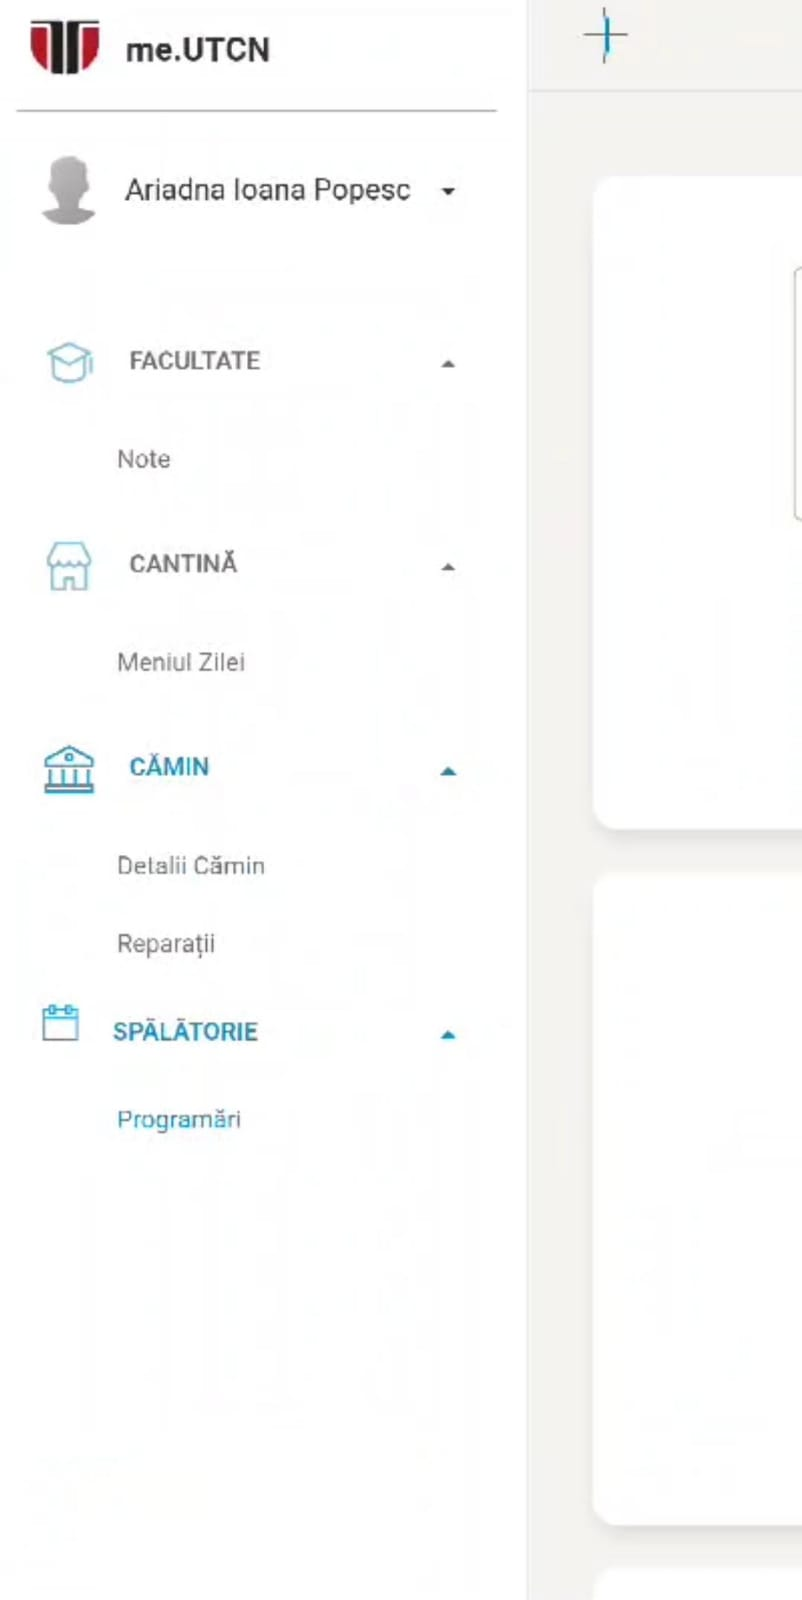
\includegraphics[width=.8\linewidth]{resurse/aplicatii_similare/utcn.png}
        \caption{Captură funcționalități}

    \end{minipage}%
    \begin{minipage}{.5\textwidth}
        \centering
        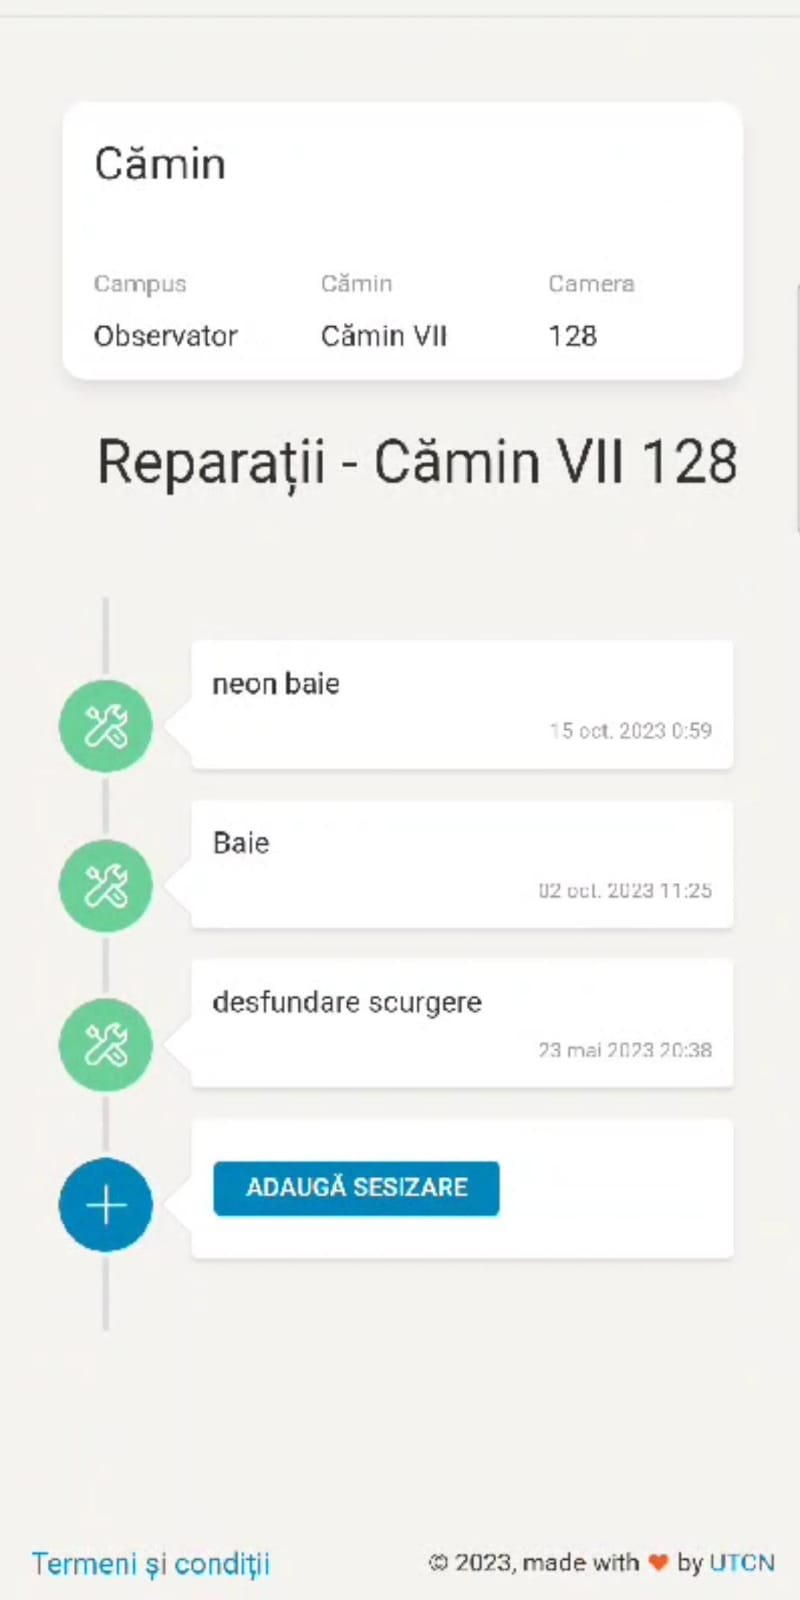
\includegraphics[width=.8\linewidth]{resurse/aplicatii_similare/utcn2.png}
        \caption{Captură formular reparații}

    \end{minipage}
\end{figure}

\subsection{TUSA }
\par TUSA (Tasmanian University Student Association)\footnote{\url{https://www.tusa.org.au/student-advocate-appointment/}}  este o aplicație destinată \textnormal{stu\-den\-ți\-lor} din cadrul Universității din Tasmania oferind sprijin pentru integrare, dar și sprijin și informații legate de resurse și servicii pentru o cât mai bună experiență studențească. Aplicația oferă informații studenților sau viitorilor studenți despre posibilele oportunități, evenimente, cluburi sau voluntariate la care pot lua parte, cum se pot înscrie  sau cum pot chiar ei să creeze un astfel de club sau societate. De asemenea, aplicația ajută studenții în ceea ce privește informarea despre beneficiile precum suport academic, consultanță financiară, alimentație sau locuințe. Studenții pot să își facă programare la mașina de spălat rufe conform orarului și disponibilității. Aceștia aleg ora și data disponibilă și își introduc numele, adresa de email și un număr de telefon. Accesul la programare nu este restricționat, deci și persoanele din afara universității pot face programare.
\par În plus, studenții sunt încurajați să ofere feedback despre experiența lor ca studenți, având o secțiune  destinată pentru acest lucru. Pentru orice întrebare sau problemă, acesția pot completa un formular în care să  detalieze nelămurirea avută.

\begin{figure}[H]
    \centering
    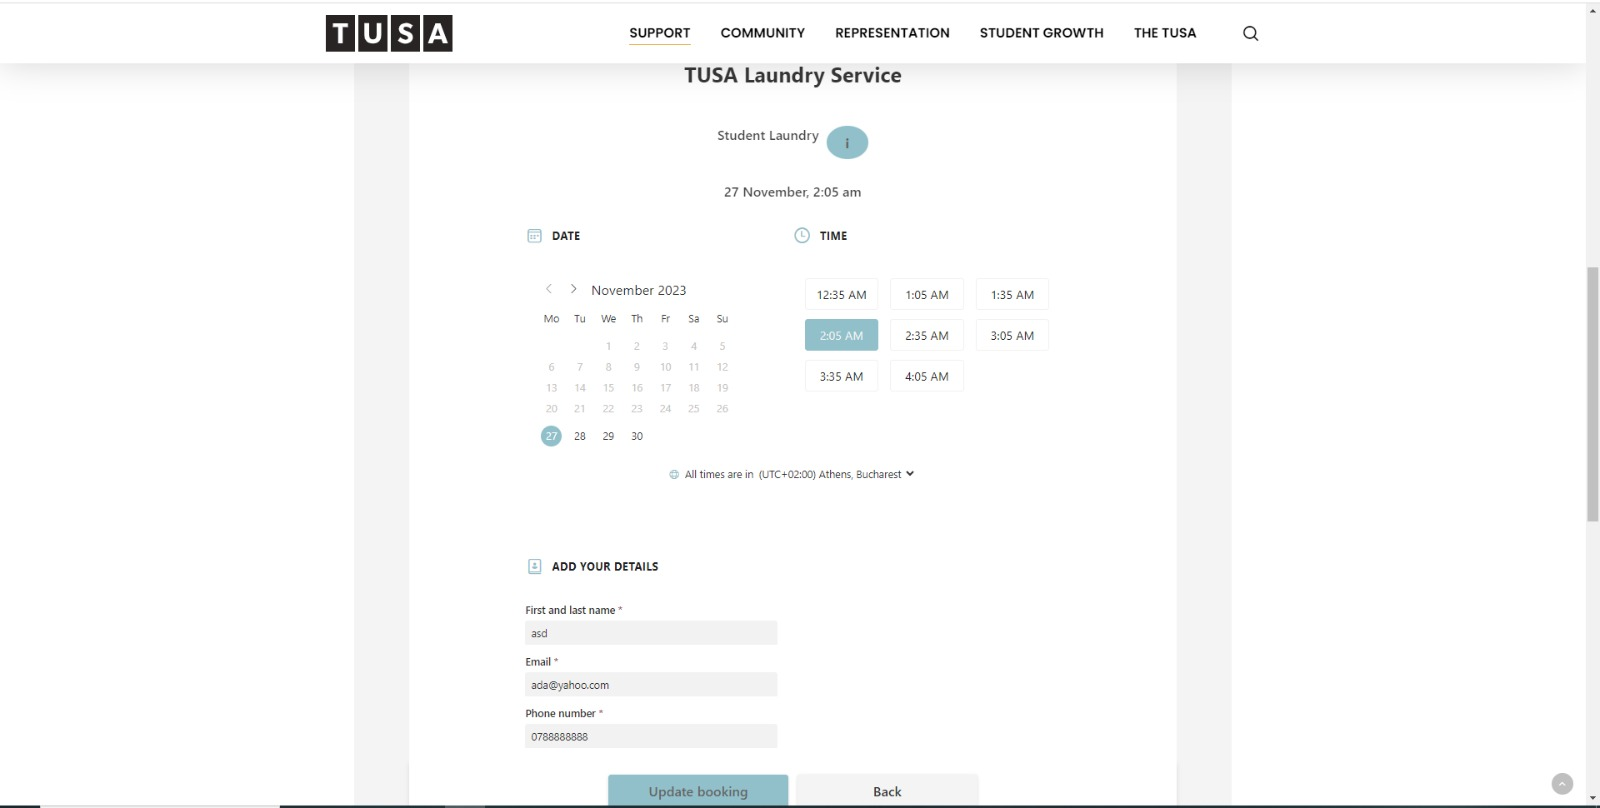
\includegraphics[scale=0.26]{resurse/aplicatii_similare/tusa.png}
    \caption{Captură programare la mașina de spălat rufe}
    \vspace{15mm}
    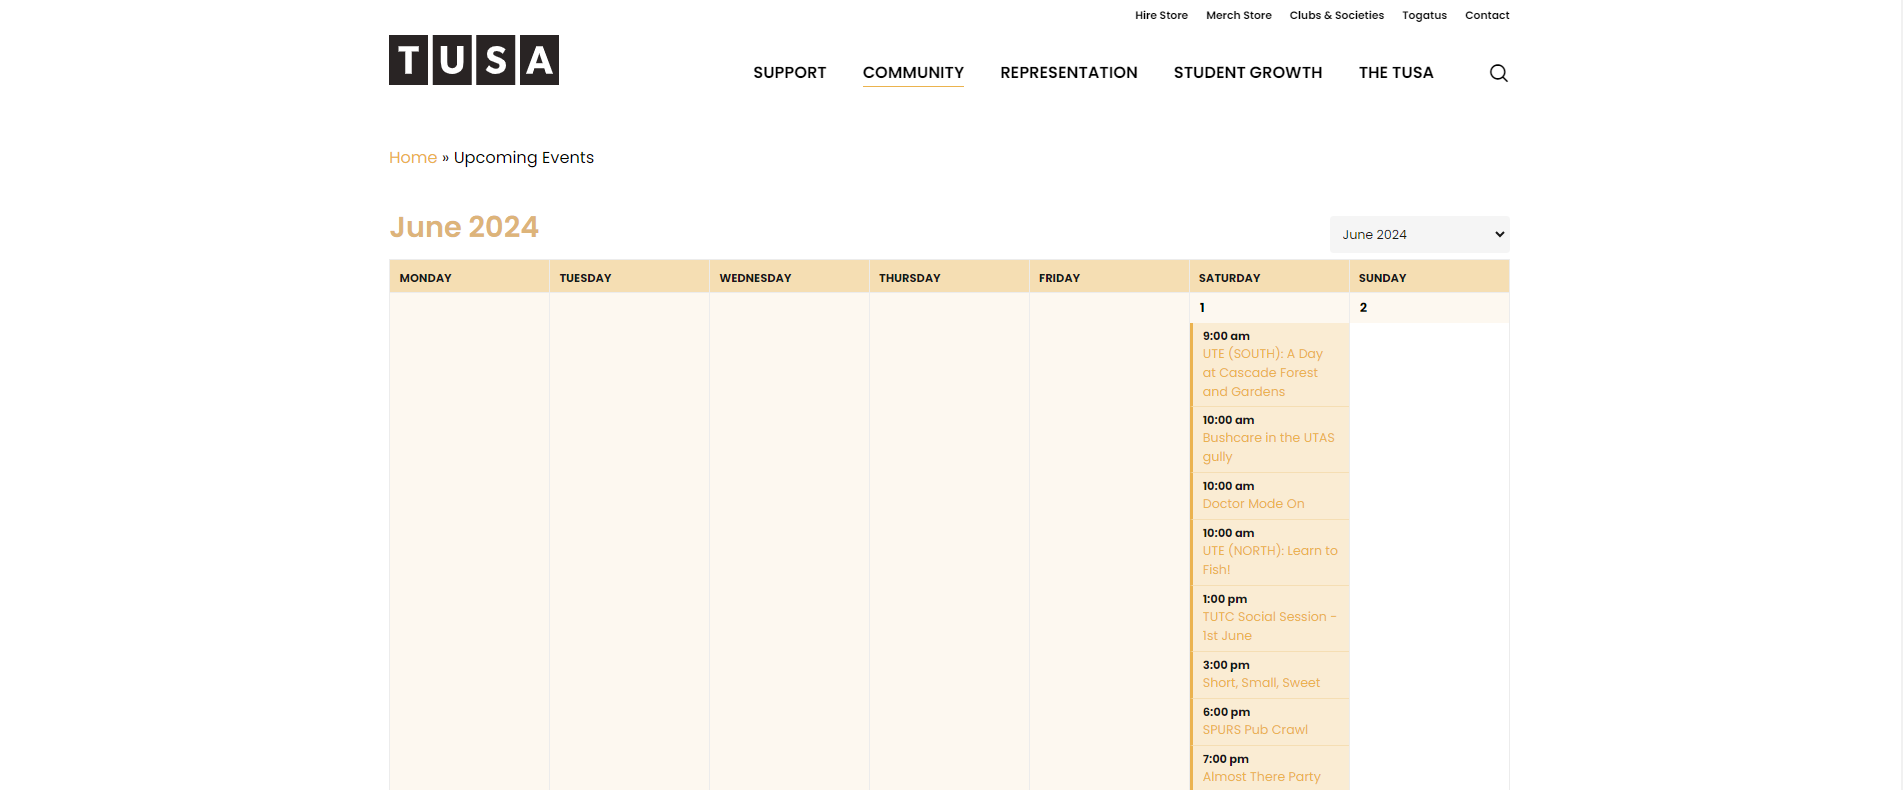
\includegraphics[scale=0.26]{resurse/aplicatii_similare/Tusa_Events.png}
    \caption{Captură evenimente}
\end{figure}

\vspace{15mm}

\section{Comparație aplicații asemănătoare}
\par Prin tabelul de mai jos, am exemplificat o scurtă comparație între cele 2 aplicații similare și UVTDorms, subliniind astfel atât punctele tari cât și punctele slabe ale fiecăreia.

\begin{table}[H]
    \centering
    \begin{tabular}{cccc}
        & \textbf{me.UTCN}         & \textbf{TUSA}  & \textbf{UVTDorms} \\
        Evenimente/anunțuri                            & Nu               & Da       &Da\\
        Feedback                                       & Nu               & Da       &Nu\\
        Formular reparații                             & Da               & Nu       &Da\\
        Validare cont                                  & Da               & Nu       &Da\\
        Programare limitată                            & Da               & Nu       &Da\\
    \end{tabular}
    \caption{Comparație între aplicații\label{comparatii-intre-aplicatii}}
\end{table}

\chapter{Arhitectura aplicației}
\par Pentru o funcționare optimă și eficientă a aplicației, arhitectura acesteia a fost gândită într-un mod care permite modularizarea componentelor principale și care prevede cele mai bune metode de intercomunicare. Arhitectura aplicației privită de la o distanță care permite înțelegarea structurării principalelor componente ale aplicației poate fi reflectată prin următoarea diagrama, așa cum poate fi observat din Figura 2.1.

\begin{figure}[H]
    \centering
    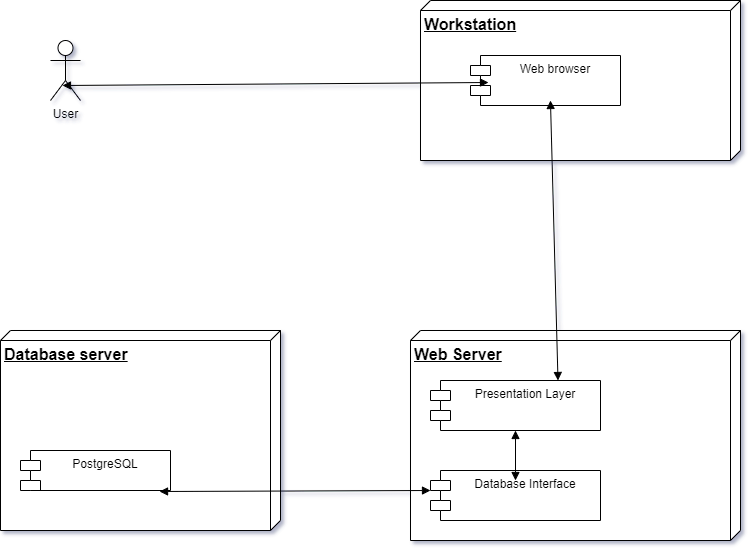
\includegraphics[width=0.75\linewidth]{resurse/diagrame/Diagrama_Arhitectura2.drawio.png}
    \caption{Diagrama arhitecturii aplicției}\label{fig:arhitect}
\end{figure}

\par Așa cum reiese și din figura\ref{fig:arhitect}, utilizatorul aplicației poate interacționa cu aceasta folosind un browser web. De asemenea, prin utilizarea infrastructurii oferite de browserele web, aplicația devine accesibilă utilizatorilor și prin utilizarea telefoanelor mobile. 

\par Browserul web este modulul care reprezintă legătura directă dintre utilizator și componenta logică și funcțională a aplicației, serverul web. Acesta oferă serviciile principale ale aplicației accesibile prin stratul de prezentare, accesat direct de browserul web prin protocolul HTTPS\@.

\par HTTPS (Hyper Text Transfer Protocol/Secure) este un protocol folosit de rețele de calculatoare. Acesta criptează datele transmise de-a lungul rețelei de la un punct la altul. Este predecesorul protocolului HTTP\@. Acesta oferă în plus securitate care se bazează pe certificatele bazate pe criptografia digitală care permite urmărirea autenticității utilizatorilor.

\par În momentul declanșării unor activități de prelucrare a datelor sau a unei cereri de date, browserul web accesează unul dintre end-point-urile stratului de prezentare a serverului web, care aplică logica funcționalității sale si returnează datele solicitate sau realizează modificările cerute.

\par Serverul web este responsabil doar pentru prelucrarea și manipularea datelor, dar nu și pentru stocarea acestora. Pentru o funcționare cât mai eficientă și optimă și pentru timp scurt de răspuns, stocarea datelor se întâmplă într-un modul separat al arhitecturii, pe serverul bazei de date, care este conectat în mod direct la serverul web prin interfața bazei de date al acesteia. Astfel, de fiecare dată când serverul web trebuie să manipuleze datele aplicației, acesta le accesează  din componenta separată.

\par Prin urmare, arhitectura aplicației este alcătuită din trei module principale, structurate într-o ierarhie de comunicare eficientă.

\section{Cazuri de utilizare}
\par Utilizatorii aplicației sunt studenții, administratorii de cămine și administratorul aplicației. Unul din cazurile de utilizare comune tuturor tipurilor de utilizatori este autentificarea care reprezintă o funcționalitate importantă prin care utilizatorii își acceseză conturile. Alături de autentificare, recuperarea parolei,schimbarea acesteia, schimbarea numărului de telefon reprezintă de asemenea, cazuri de utilizare comune. Recuperarea parolei reprezintă o măsură de siguranță în cazul în care utilizatorul își pierde parola, ceea ce ar însemna și imposibilitatea de a accesa contul. Prin această funcționalitate, utilizatorii au posibilitatea de a-și salva contul și de a-și seta o parolă nouă. De asemenea, schimbarea parolei este posibilă și în cazuri generale din meniul de setări a tuturor tipurilor de utilizatori ca o formă de siguranță.

\begin{figure}[H]
    \centering
    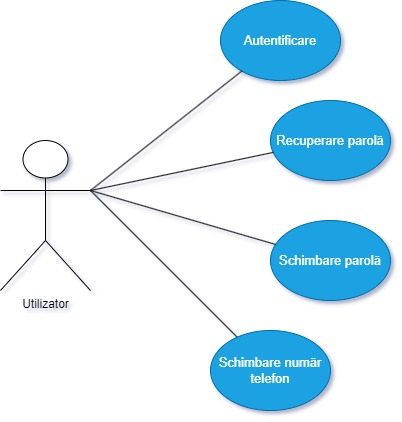
\includegraphics[width=0.5\linewidth, height=0.3\textheight]{resurse/diagrame/UVTDorms_UseCase_Student.jpg}
    \caption{Diagrama cazuri de utilizare comune}
\end{figure}

\par Cazurile de utilizare sunt reprezentate și detaliate pentru fiecare tip de utilizator în subsecțiunile următoare.

\subsection{Cazuri de utilizare pentru student}
\par Principalul beneficiar al aplicației web este studentul locatar în căminul studențesc. Odată cazat în cămin, acesta poate să își creeze un cont și să solicite administratorului căminului din care face parte, validarea contului de student asociat cu căminul respectiv. După crearea cererii, studentul primește un mail de confirmare cu privirea la realizarea cererii de înscriere și o parolă temporală pentru cont, pe care o poate schimba ulterior. Până la acceptarea cererii de înscriere, poate să intre în aplicație cu email-ul cu care și-a creat contul și parola primită, dar nu va avea acces la funcționalitățiile oferite, rolul acestuia fiind de student inactiv.

\par Una dintre principalele funcționalități dedicată studenților este crearea \textnormal{pro\-gra\-mă\-ri\-lor} la spălătoria căminului. Aceștia pot beneficia de o programare săptămânală, care este formată din două ore la mașina de spălat rufe urmate de două ore la uscătorul de rufe. În cazul în care studentul dorește anularea programării, acesta poate anula programarea și, în limita disponibilităților, să realizeze o altă programare. Dacă pe perioada șederii în căminul studențesc apar diferite probleme tehnice care necesită intervenție din partea personalului, aceștia pot crea un tichet pentru reparații.

\par De asemenea, propagarea în mod eficient a informațiilor despre evenimentele ce au loc în cadrul căminului este asigurată de funcționalitățile organizatorice specifice.

\begin{figure}[H]
    \centering
    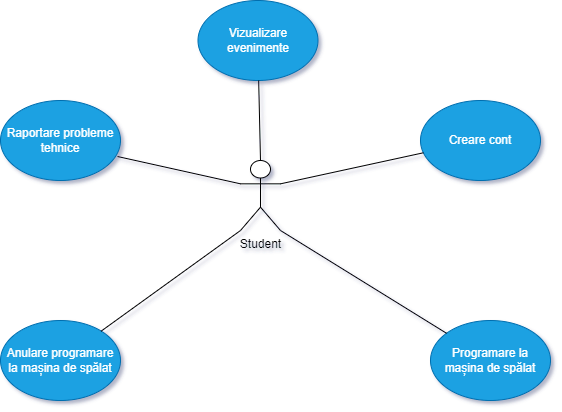
\includegraphics[width=0.75\linewidth]{resurse/diagrame/use_case_student.drawio.png}
    \caption{Diagrama cazuri de utilizare student}
\end{figure}

\subsection{Cazuri de utilizare pentru administratorul de cămin}
\par Administratorul de cămin are unul dintre cele două roluri de administrare ale aplicației, care este responsabil pentru administrarea unui cămin și al studenților cazați în căminul respectiv.

\par Acest rol prevede manipularea listei studenților în perioada de înscriere, adică acceptarea sau respingerea studenților care au un loc într-un cămin, sau dezactivarea conturilor studenților asociate căminului. Tot printre responsabilitățile administratorului se află și organizarea spălătoriei din cămin, adică administrarea mașinilor de spălat și a uscătoarelor de rufe, și administrarea programărilor. În cazul în care apare o problemă tehnică în cămin, și un tichet de reparații a fost deschis, administratorul este responsabil să se ocupe de acesta și, în cazul în care e necesar, să creeze anunțuri care ajung la toți studenții afectați.

\par Pe lângă cele descrise mai sus, administrarea evenimentelor ce au loc în cadrul căminului, se află tot pe lista responsabilităților administratorului căminului, care le poate crea, edita și șterge.

\begin{figure}[H]
    \centering
    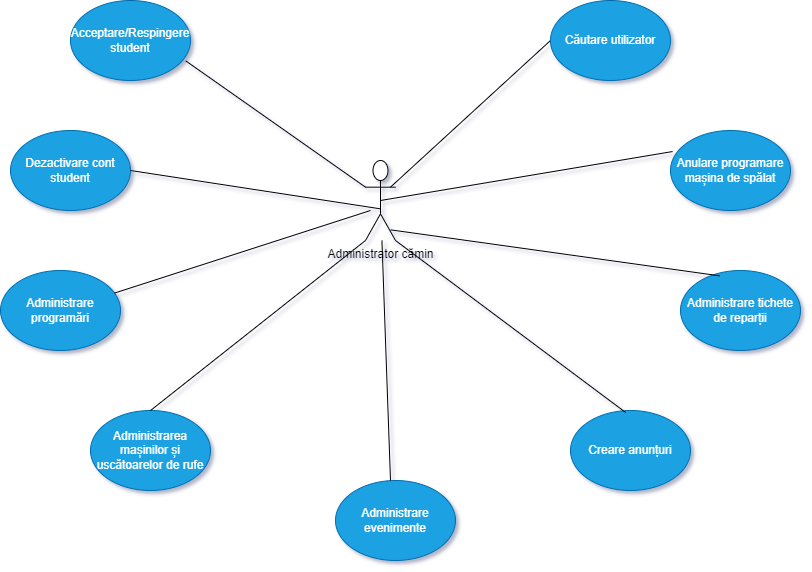
\includegraphics[width=0.75\linewidth]{resurse/diagrame/Usecase_administrator_camin.drawio.png}
    \caption{Diagrama cazuri de utilizare administrator cămin}
\end{figure}

\subsection{Cazuri de utilizare pentru administratorul aplicației}
\par Administrarea la nivel înalt al aplicației este o activitate crucială în origanizarea aplicației. Acest rol prevede atât responsabilități legate de căminele universității care folosesc aplicația, cât și cele legate de administratorii acestor cămine.

\par Astfel, unul dintre principalele cazuri de utilizare ale administratorilor de aplicație este adăugarea de cămin, prin care sistemul căminelor universității poate fi extins.

\par Căminelor existente în sistem, administratorul aplicației le poate asocia câte un administrator. Totodată, și schimbarea administratorilor se realizează de administratorul aplicației. În acest caz, contul administratorului de cămin nu este șters, ci doar dezactivat de administratorul aplicației.

\begin{figure}[H]
    \centering
    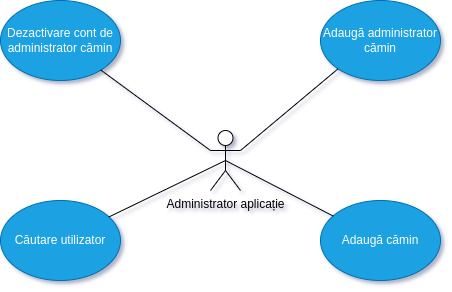
\includegraphics[width=0.75\linewidth]{resurse/diagrame/cazuri_de_utilizare_administrator_aplicatie_1.png}
    \caption{Diagrama cazuri de utilizare administrator cămin}
\end{figure}

\section{Structura unităților de execuție}
\par Așa cum s-a putut observa și din diagrama de instalare prezentată mai sus, aplicația este structurată pe mai multe straturi, care la rândul lor sunt modularizate pentru o funcționare logică și eficientă.

\par Primul modul, cel al clientului, este alcătuit din trei componente ale căror cooperare oferă o experință plăcută utilizatorului, fiind modulul care interacționează în mod direct cu acesta. Prima componentă, HTML GUI constituie interfața aplicției cu care ia contact utilizatorul declanșând acțiunile care reprezintă funcționalitățile aplicției prin elemente de HTML precum butoane. Aceste acțiuni declanșate de componenta HTML GUI sunt reprezentate de componenta GUI function. Cea de-a doua componentă (GUI function) este responsabilă pentru activitățile logice ale primului modul și declanșează inițierea legăturii cu următorul modul prin cea de-a treia componentă, Client-Side Angular Services.

\par Cel de al doilea modul, este structurat în patru componente care sunt responsabile pentru diferite activități de execuție. Controller-ul, este componenta care \textnormal{in\-te\-rac\-ți\-o\-nea\-ză} în mod direct cu primul modul și conține end-point-urile care sunt accesate de  Client-Side Angular Services. În cea de a doua componentă, Services, se realizează logica de afaceri bazată pe datele primite de la utilizator. JPA Repository este componenta care interacționează în mod direct cu baza de date, oferind funcții de manipulare a datelor utilizând reprezentările interne ale tabelelor. Acestea sunt create cu ajutorul mapării entitatăților din componenta Entity.

\par Ultimul modul, DataBase Server este responsabil pentru stocarea, structurarea și organizarea datelor, astfel încât accesarea lor să fie posibilă într-un mod cât mai eficient.

\begin{figure}[H]
    \centering
    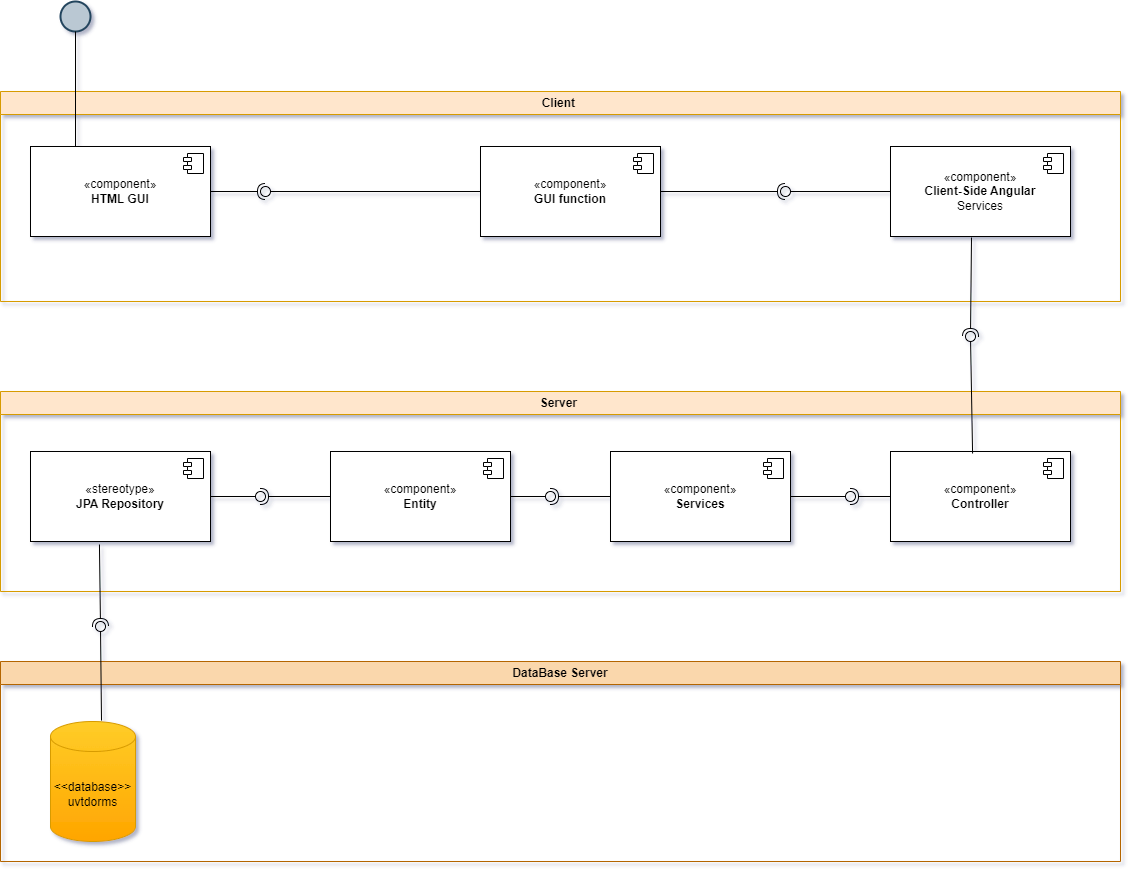
\includegraphics[width=0.75\linewidth]{resurse/diagrame/DiagramaDEEXECUTIE.drawio.png}
    \caption{Diagrama unităților de execuție}
\end{figure}

\section{Structura bazei de date}\label{sec:architectura-bazei-de-date}
\par Având în vedere varietatea obiectelor abstracte pe care le folosește sistemul, și necesitatea de reutilizare a acestora, aplicația își are datele structurate într-o bază de date. Toate elementele din această structură încapsulează informații esențiale despre principalele obiecte cu care operează aplicația.

\par Una dintre cele mai importante abstractizări este cea al userului, tabelul \textit{users}, care este o structură ce încapsulează datele unui utilizator obișnuit, cum ar fi numele, adresa de e-mail, numărul de telefon, parola, rolul, starea de activitate a contului și, desigur, un identificator unic.

\par Printre tipurile de utilizatori se enumără și studenții, care au anumite date pe care restul tipurilor de utilizatori nu le au, motiv pentru care a fost nevoie crearea unei tabele, \textit{students\_details}, care are ca atribute detaliile necesare lucrării cu obiecte ce abstractizează studenți. Printre aceste detalii se află CNP-ul, identificatorul unic al camerei în care este cazat studentul și numărul matricol.

\par Un alt tip de utilizator cu detalii diferite este administratorul căminului, care, pe lângă datele unui utilizator obișnuit, mai are și identificatorul unic al căminului pentru care este responsabil. Pentru încapsularea acestor informații am creat tabelul \textit{dorm\_administrator\_details}.q

\par Anunțurile din sistem sunt încapsulate în tabelul \textit{announcements}, care are un identificator unic al anunțului, identificatorul unic al utilizatorului care a creat anunțul, un titlu, un text ce reprezintă descrierea anunțului și data in care anunțul a fost creat.

\par Căminele aflate în sistem au fiecare un identificator unic, o adresă și un nume, încapsulate în tabelul \textit{dorms}. Camerele din cămine au într-un mod similar un identificator unic, numărul camerei în contextul căminului și identificatorul unic al căminului, în tabelul \textit{rooms}.

\par Datele mașinilor de spălat și ale uscătoarelor din spălătoriile căminelor sunt în tabelele \textit{wash\_machines} și \textit{dryers}. Ambele au un identificator unic, la fel și identificatorul unic al căminului în care se află, un număr de identificare în contextul căminului și un câmp care reprezintă starea mașinii, adică disponibilitatea acesteia, sau dacă este defectă.

\par Programările la spălătoria căminului sunt reprezentate prin structura tabelului \textit{laundry\_appointments}. Fiecare programare are un identificator unic, precum și identificatorul unic al utilizatorului care a creat-o, dar și identificatoarele unice al mașinii de spălat și al uscătorului la care s-a făcut programarea. Începutul și finalul rezervării sunt informații care sunt încapsulate tot în această structură.

\section{Structura unităților de cod}
\par Mai jos sunt prezentate diagramele unităților de cod. Acestea reflectă structurarea codului care implementează funcționalitățile și serviciile serverului web, precum și mapările care permint conectarea la baza de date.

\par Entitățile existente în cod sunt mapările directe ale elementelor din baza de date în care se specifică explicit încapsularea internă dintre ele, ca și consecință a relațiilor. Prin urmare, în diagrama din Figura 2.7.\ putem observa relații bidirecționale, de compoziție și agregare. De exemplu, relația de compoziție dintre \textit{User} și \textit{StudentDetails}, unde cel din urmă are mereu un obiect de tip \textit{User}. Dar această relație în contextul entităților presupune și un complement al relației de compoziție, în cazul nostru cea de agregare care se realizează printr-o listă de obiecte de tip \textit{StudentDetails} în contextul \textit{User}.

\begin{figure}[H]
    \centering
    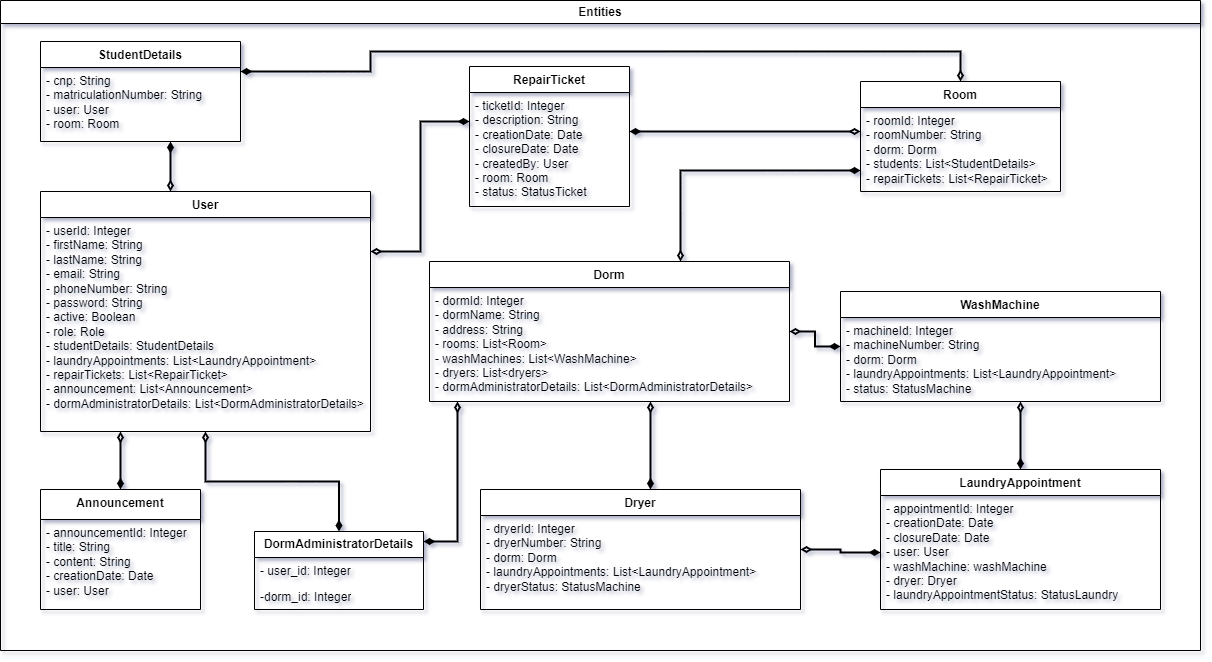
\includegraphics[width=1\linewidth]{resurse/diagrame/uvtdorms1.2.drawio.png}
    \caption{Diagrama unităților de cod pentru entități}
\end{figure}

\par Repository reprezintă stratul de abstractizare a bazei de date. JPA Repository pune la dispoziție diferite metode specializate pe manipularea tabelelor existente în baza de date precum scrierea, ștergerea și modificarea datelor. În același timp, \textnormal{re\-po\-si\-to\-ry-urile} permit definirea unor metode specifice pentru executare unor operații complexe.

\begin{figure}[H]
    \centering
    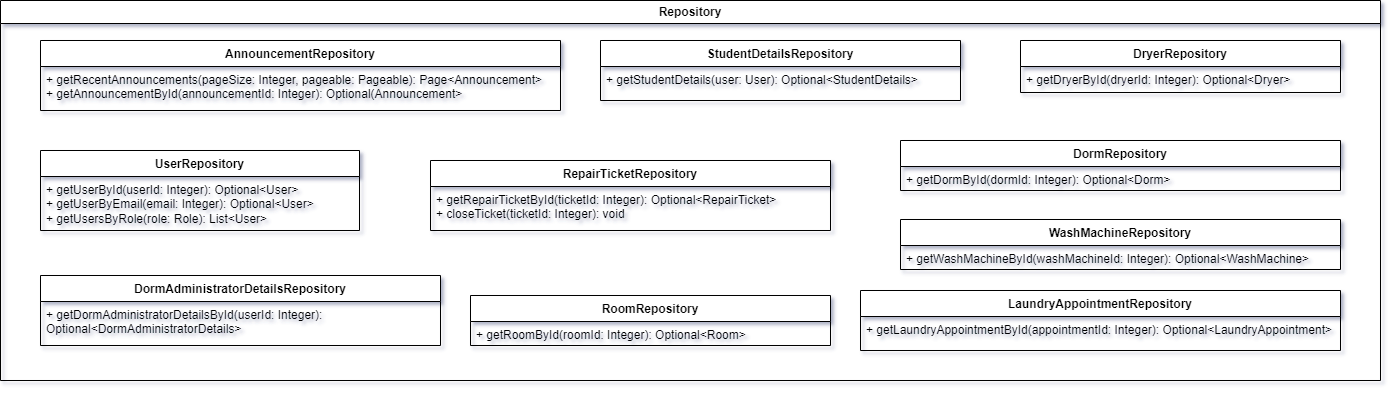
\includegraphics[width=1\linewidth]{resurse/diagrame/uvtdorms_d2.drawio.png}
    \caption{Diagrama unităților de cod pentru repository}
\end{figure}

\par Serviciile corespunzătoare fiecărei componente din sistem sunt elementele cheie în manipularea obiectelor existente. Ele sunt responsabile pentru activitățile principale și execută operații complexe, uneori folosindu-se chiar de alte servicii. De exemplu, \textit{LaundryAppointmentService} utilizează numeroase alte servicii pentru realizarea cererilor legate de programările la spălătorie.

\begin{figure}[H]
    \centering
    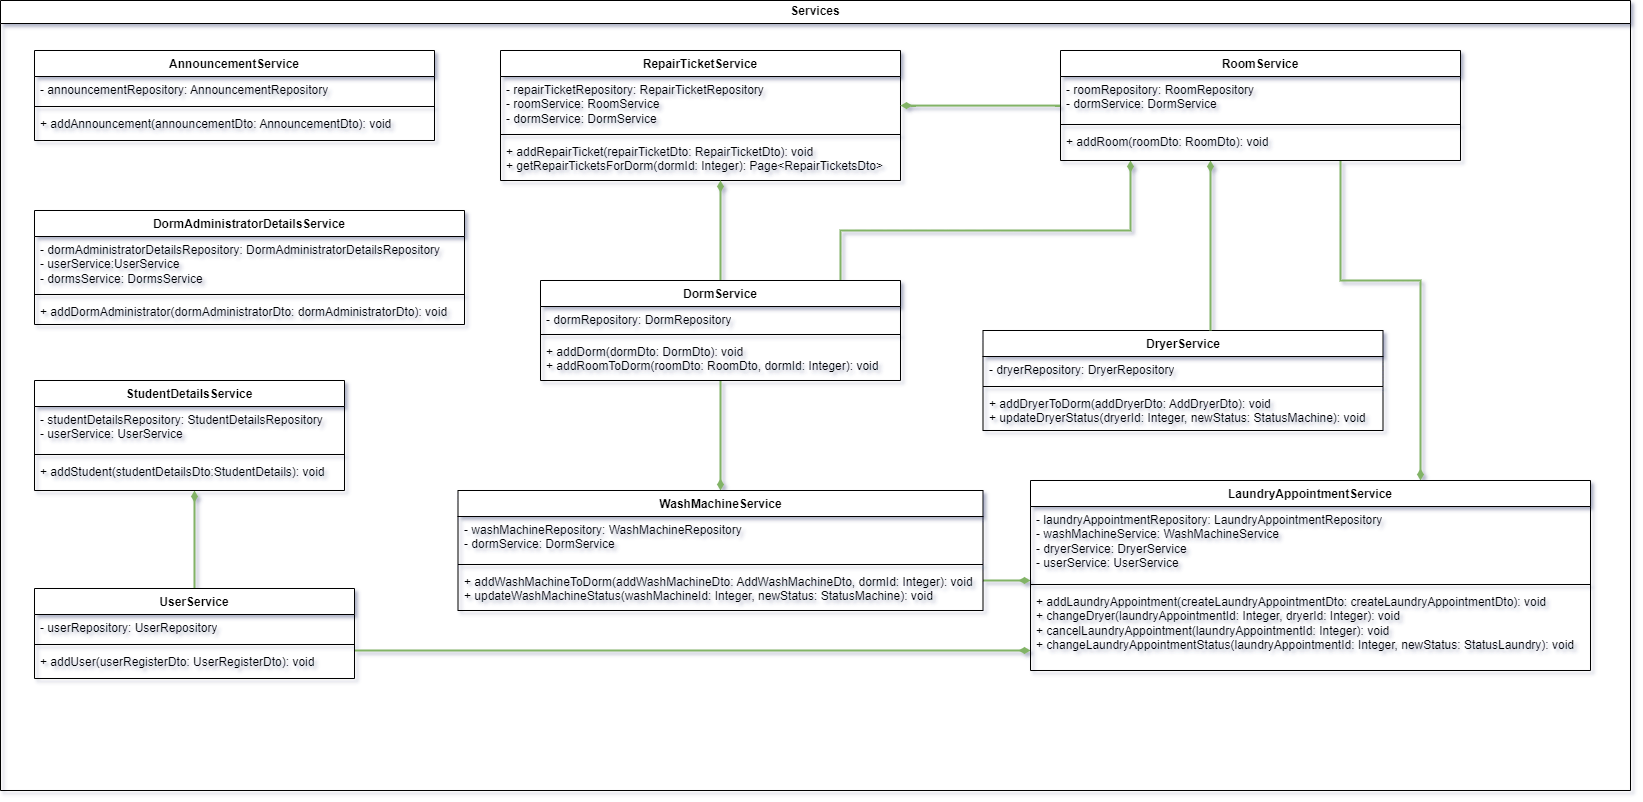
\includegraphics[width=1\linewidth]{resurse/diagrame/uvtdorms_d3.drawio.png}
    \caption{Diagrama unităților de cod pentru servicii}
\end{figure}

\par Controllerele reprezintă end-point-urile serverului web ale aplicație și oferă metode predefinite care execută operații solicitate de client. Controllerele au fiecare un service la care redirecționează apelurile venite din exterior.

\begin{figure}[H]
    \centering
    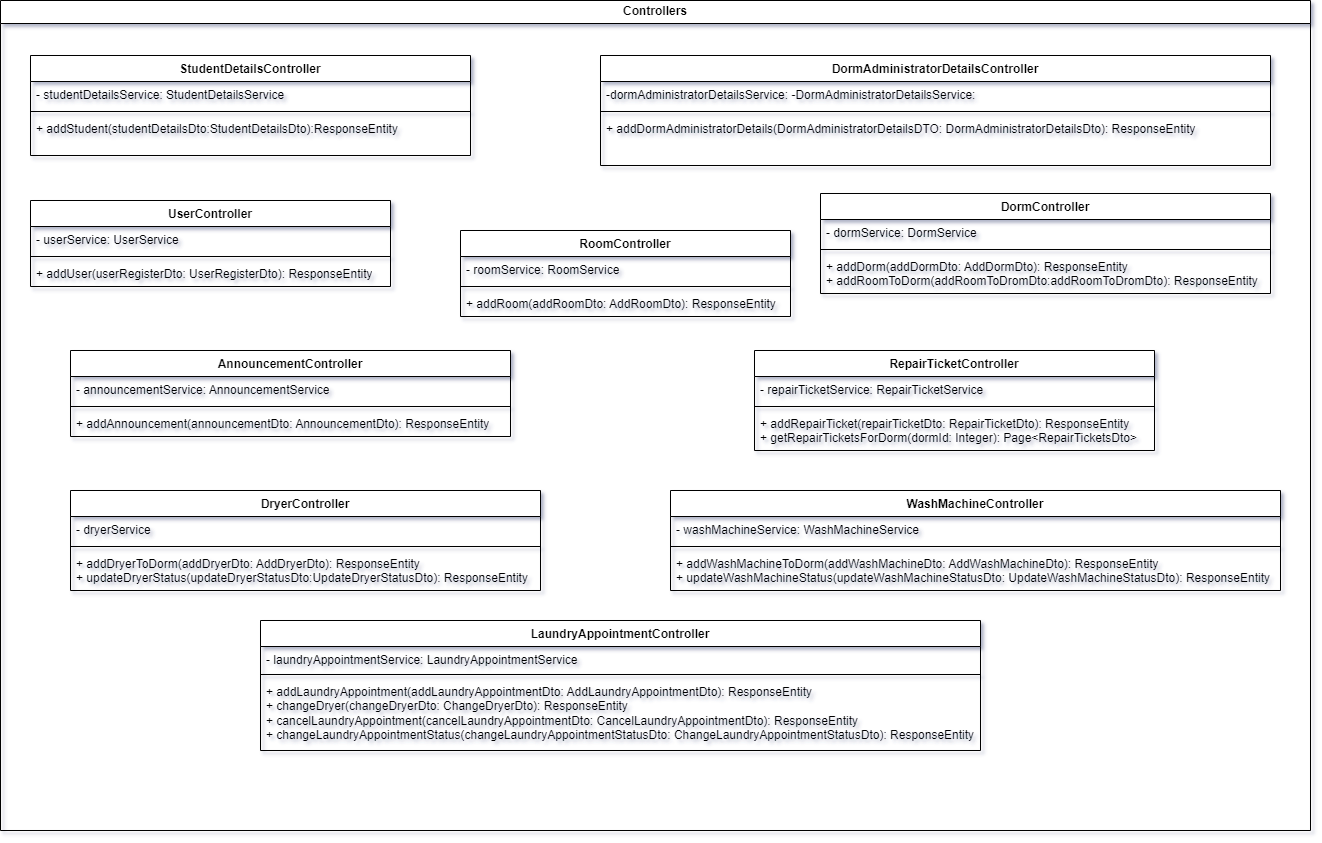
\includegraphics[width=1\linewidth]{resurse/diagrame/uvtdorms_d4.drawio.png}
    \caption{Diagrama unităților de cod pentru controllere}
\end{figure}

\section{Flux de navigare}
\par Fluxul de navigare al aplicației a fost gândit să fie unul intuitiv, ușor de folosit pentru oricine. Prin urmare, în loc de pagini multiple și pași complecși de navigare, am ales o structura simplă a paginilor.

\par Având în vedere că aplicația are mai multe tipuri de utilizatori, paginile accesibile de aceștia diferă și, prin urmare, la fel și fluxul de navigare. Însă, un element ce poate fi regăsit în fluxul oricărui utilizator este pagina de autentificare, punctul în care se întâmplă divergența ramurilor fluxurilor de navigare, unde se poate verifica tipul utilizatorului.

\par În cazul în care utilizatorul încă nu are un cont, poate intra pe pagina de înregistrare care, la fel ca pagina de autentificare, este accesibilă tuturor tipurilor de utilizatori, apăsând pe butonul de înregistrare aflată pe pagina de autentificare. După ce formularul de înregistrare a fost completat și butonul de finalizare apăsat, utilizatorul este redirecționat pe pagina de autentificare prin butonul cu mesajul sugestiv, ce apare pe pop-up-ul posterior finalizării completării formularului de înregistrare.

\par În momentul în care utilizatorul s-a autentificat, acesta este redirecționat pe pagina acasă. De acolo poate reveni pe pagina de autentificare apăsând pe butonul de delogare. Pagina acasă afișează informații generale, dar și butoane diferite în funcție de tipul utilizatorului. Însă, butonul care redirecționează utilizatorul pe pagina cu detaliile contului este vizibilă pentru toate tipurile de utilizatori.

\par Pagina cu detaliile contului utilizatorului afișează istoricul activităților acestuia și opțiunile de setare a datelor, precum parola. De aici, utilizatorul poate reveni pe pagina acasă apăsând pe butonul cu același nume.

\subsection{Fluxul de navigare din perspectiva unui student}
\par Studenții sunt cei care au acces la paginile care întruchipează principalele \textnormal{func\-ți\-o\-na\-li\-tăți} ale aplicației.

\par Una dintre aceste pagini este pagina de crearea programărilor la spălătorie, accesibilă prin butonul \textit{creare programare} aflat pe pagina acasă. Pentru a face o programare, studenții trebuie să completeze un formular unde tebuie să seteze informații legate de programare, precum data și intervalul în care are loc aceasta și mașina de spălat la care se face programarea. După finalizarea completării formularului, în urma apăsării butonului de finalizare, apare pop-up-ul de confirmare a creării programării cu un buton de redirecționare pe pagina acasă.

\par O altă pagină accesibilă doar studenților este pagina de raportare de probleme tehnice. Aici studentul poate furniza informații despre camera sau căminul în care a fost identificată problema (în cazul în care problema nu se află într-o cameră a căminului, atunci se specifică doar căminul), data identificării acesteia, descrierea problemei și alte informații relevante. După trimiterea raportului, apare un pop-up care confirmă crearea acestuia, alături de un buton de redirecționare pe pagina acasă.

\par Pentru vizualizarea evenimentelor ce au loc în cadrul căminului, studenților se află la dispoziție pagina de evenimente, unde pot afla detaliile activităților. De aici, se pot întoarce pe pagina de acasă cu ajutorului butonului cu același nume.

\begin{figure}[H]
    \centering
    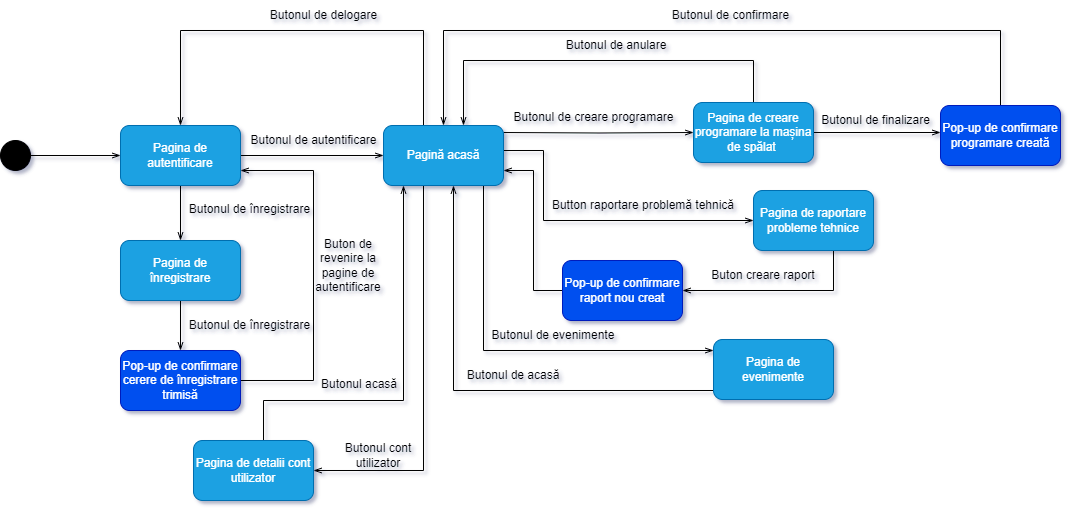
\includegraphics[width=0.75\linewidth]{resurse/diagrame/diagrama_de_navigare1.1.drawio.png}
    \caption{Diagrama de stări și tranziții cu fluxul ecranelor pentru student}
\end{figure}

\subsection{Fluxul de navigare din perspectiva unui administrator cămin}
\par Administratorul căminului este responsabil pentru majoritatea elementelor organizatorice din cadrul unui cămin. Prin urmare, acesta are acces la numeroase pagini de administrare, de unde poate reveni pe pagina acasă cu ajutorului butonului \textit{acasă}.

\par Una dintre paginile de administrare este cea a studenților, unde administratorul căminului poate accepta sau respinge studenții care s-au înregistrat la un cămin. Tot aici, administratorul poate să efectueze căutări în lista studenților cazați în cămin și mai are și opțiuni de a inactiva conturile studenților.

\par Pentru adăugarea sau aplicarea stării de indisponibiliate a mașinilor din spălătoria căminului și administrarea altor utilități din cămin, administratorul are la dispoziție pagina de administrare a căminului, accesibilă prin butonul \textit{cămin}.

\par Pagina de administrare programări, accesibilă prin butonul \textit{programări}, afișează detaliile legate de programările la spălătoria căminului precum și istoricul de programări. Aici administratorul are opțiunea de a urmări demersul acestora și opțiunea de a anula programări.

\par Pentru administrarea raportărilor problemelor tehnice, administratorul căminului are acces la o pagină dedicată, prin butonul \textit{raportări probleme tehnice}, unde poate vedea detaliile rapoartelor și le poate închide după ce acestea au fost rezolvate.

\par Ultima pagină administrativă ce se află la dispoziția administratorului este cea a evenimentelor, pe care poate intra apăsând pe butonul \textit{evenimente}. Aici administratorul poate crea, modifica și șterge evenimente ce au loc în cadrul căminului.

\begin{figure}[H]
    \centering
    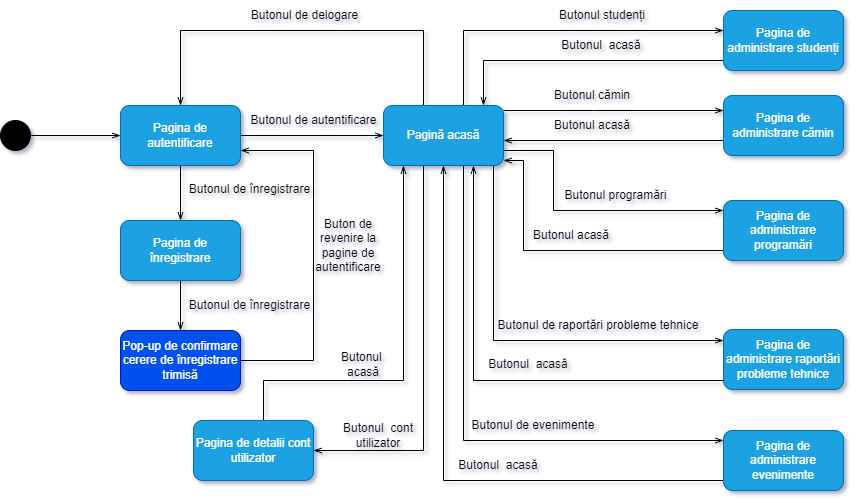
\includegraphics[width=0.75\linewidth]{resurse/diagrame/diagrama_de_navigare.2drawio.png}
    \caption{Diagrama de stări și tranziții cu fluxul ecranelor pentru administartorul de cămin}
\end{figure}

\subsection{Fluxul de navigare din perspectiva administratorului aplicției}
\par Administrartorul aplicației este cel care se ocupă atât de buna funcționare a \textnormal{ap\-li\-ca\-ți\-ei}, cât și de adăugarea căminelor și distribuirea noilor administratori.

\par Acesta prin butonul \textit{administratori} poate accesa pagina unde are posibilitatea de a vizualiza și  a realiza diferite operații asupra administratorilor de cămine, precum adăugarea și inactivarea conturilor administratorilor sau căutarea acestora. Tot aici, odată adăugați administratorii, acestora li se pot atribui căminul corespunzător.

\par Pentru administrarea căminelor, administratorul aplicației are acces la pagina cu același nume prin intermediul butonului \textit{cămine}, unde poate adăuga sau șterge cămine.

\begin{figure}[H]
    \centering
    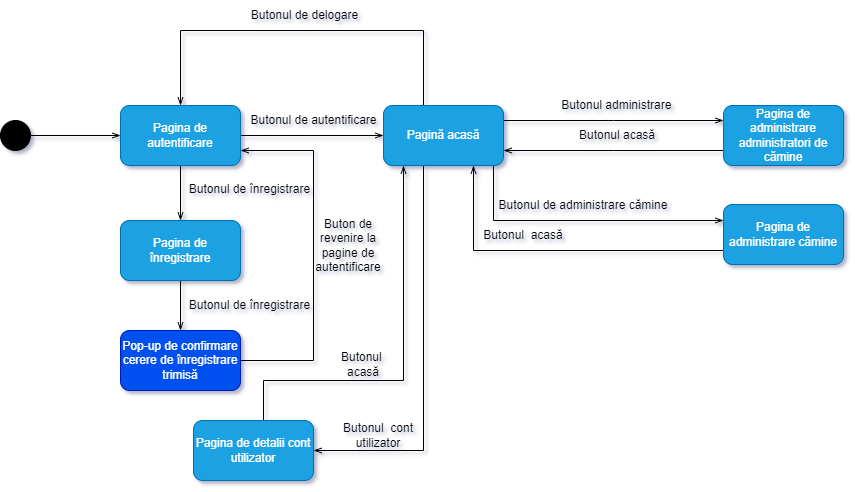
\includegraphics[width=0.75\linewidth]{resurse/diagrame/diagrama_de_navigare3.drawio.png}
    \caption{Diagrama de stări și tranziții cu fluxul ecranelor pentru administratorul aplicației}
\end{figure}

\chapter{Implementarea aplicației}
\par Pentru realizarea propriu-zisă a aplicației voi urmări structura prezentată în capitolul anterior. Dezvoltarea se va desfășura în paralel atât pe partea de front-end a aplicației, cât și pe partea de back-end. Astfel, fiecare funcționalitate va fi implementată incremental, iar testarea lor va fi posibilă și din perspectiva utilizatorului, deja de la începutul dezvoltării.

\par Având în vedere că implementarea unor mecanisme sunt similare, vor fi prezentate doar câte un exemplar din cele distincte. Deși pe parcursul realizării codului sursă se urmăresc pincipiile \textit{Clean Code}\cite{martin2009clean} și se evită repetarea codului și se profită de avantajele programării orientate obiect, este totuși imposibilă modularizarea microserviciilor astfel încăt să nu existe părți similare.

\section{Configurarea backend-ului}
\par Printre lucrurile prioritare în dezvoltarea aplicației se află realizarea conexiunii dintre front-end și back-end. Acesta presupune mai mulți factori, principalele fiind de natură de securitate. Framework-ul Spring-Boot permite variate configurații ale serverului pentru a asigura accesarea serviciilor doar de cei autorizați, creând astfel măsurile de bază ale securității aplicației\cite{scarioni2019pro}.

\par În secțiunile următoare vor fi prezentate configurarea accesului la serviciile serverului atât prin condiționarea adreselor care solicită acces, cât și prin condiționarea accesurilor prin verificarea parametrilor din solicitare. Cel din urmă va fi executată doar în cazul anumitor puncte de acces, fiindcă serverul va avea și servicii \textit{publice}, adică servicii care sunt accesibile nu numai utilizatorilor care au un cont.

\subsection{Cross-Origin Resource Sharing}
\par Unul dintre cele mai aplicate mecanisme de filtrarea apelurilor este \textit{Cross-Origin Resource Sharing}\cite{gibbinscross} (CORS). Acesta vine cu funcționalități diferite în funcție de nivelul de aplicabilitate.

\par La nivelul protocolului, CORS adaugă un câmp nou în header-ul cererilor, care indică originea solicitării de acces. Astfel, pot fi restricționate originile de la care serverul să accepte cereri. Tot aici, pot fi specificate și tipul cererilor ce se pot face pentru back-end (GET, PUT, OPTIONS, etc.).

\par La nivel de API (Application Programming Interface) cererile restricționate vor primi totuși un răspuns, generat de browser. Un mesaj de eroare se generează în cazul cererilor respinse, dar acesta nu este accesibil din script, doar apare în consolă.

\begin{figure}[H]
    \centering
    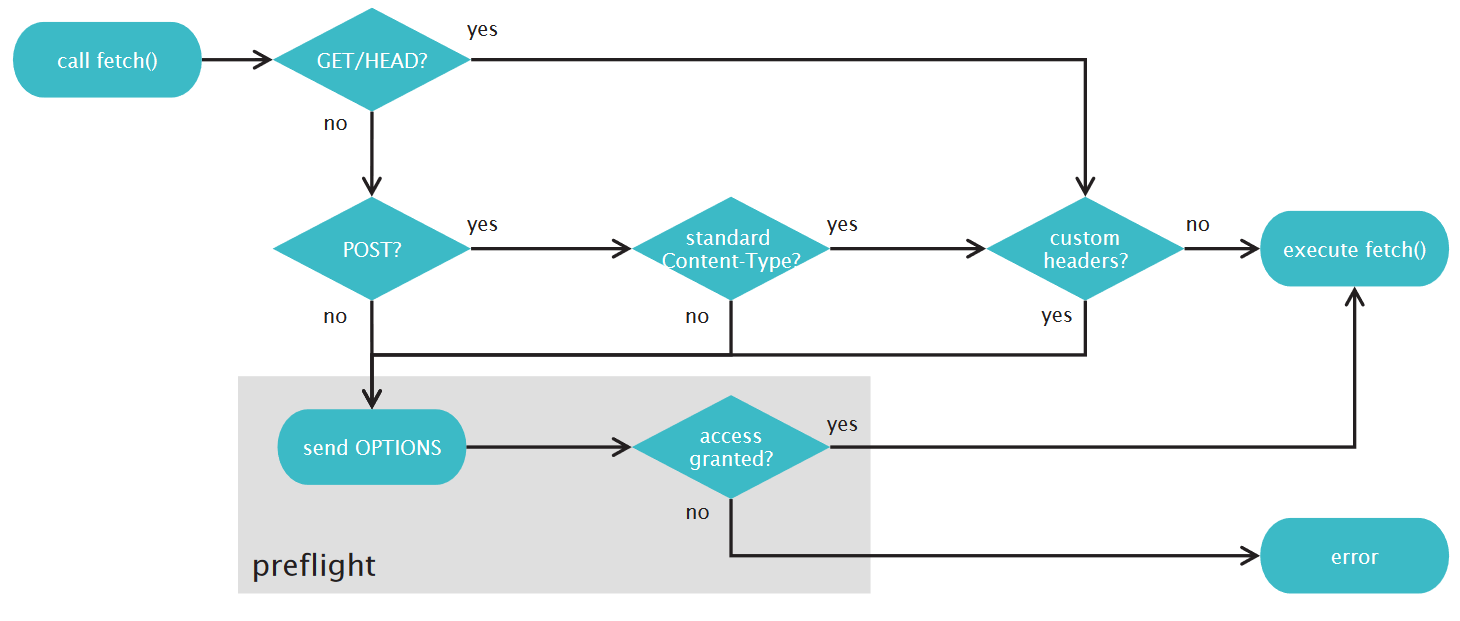
\includegraphics[width=1\linewidth]{resurse/diagrame/diagrama_cors.png}
    \caption{CORS flow\cite{gibbinscross}}
\end{figure}

\par Pentru a configura CORS pentru aplicația UVTDorms, se va crea clasa \textit{`CorsConfig'} în folderul \textit{`utils/'}. Clasa va avea un \textit{`@Bean'}, adică o funcție ce va returna un obiect de tip \textit{`CorsFilter'}. Aici va fi creată sursa ce permite configurarea CORS pe baza URL-lui. Configurarea va acoperi aspecte cum ar fi:

\begin{enumerate}
    \item configurarea originilor cu acces (pe parcursul dezvoltării, singurul URL cu acces va fi \textit{`http://localhost:4200'})
    \item configurarea tipurilor de header permise
    \item specificatea metodelor permise
    \item setarea punctelor de acces pentru care se aplică configurarea cors (pentru a include toate punctele, se va da URL-ul \textit{`/**'})
\end{enumerate}

\begin{lstlisting}[language=Java, caption={Clasa prin care se realizează configurarea CORS}]
@Configuration
@EnableWebMvc
public class CorsConfig
{
    @Bean
    public CorsFilter corsFilter(){
        UrlBasedCorsConfigurationSource source= new UrlBasedCorsConfigurationSource();
        CorsConfiguration config = new CorsConfiguration();
        config.setAllowCredentials(true);
        config.addAllowedOrigin("http://localhost:4200");
        config.setAllowedHeaders(Arrays.asList(
                HttpHeaders.AUTHORIZATION,
                HttpHeaders.CONTENT_TYPE,
                HttpHeaders.ACCEPT
        ));
        config.setAllowedMethods(Arrays.asList(
                HttpMethod.GET.name(),
                HttpMethod.POST.name(),
                HttpMethod.PUT.name(),
                HttpMethod.DELETE.name()
        ));
        config.setMaxAge(3600L);
        source.registerCorsConfiguration("/**",config);

        return new CorsFilter(source);
    }
}
\end{lstlisting}

\subsection{JSON Web Token Authentification}
\par Una dintre cele mai sigure metode de autentificare și de încapsulare a anumitor informații relevante este JSON Web Token\cite{jones2015json}. Acesta este un token care, de fapt reprezintă un obiect JSON criptat. În mod normal, aceste obiecte conțin informații necesare la autentificarea utilizatorilor. Deoarece este criptat, token-ul poate fi salvat local, în cache-ul browser-ului și poate fi citit la următoarea accesare a aplicației web.

\par În cadrul aplicației UVTDorms, obiectul JSON criptat conține o cheie de autentificare temporară, rolul și adresa de email ale utilizatorului. Token-ul obținut prin criptarea obiectului este inclus în header-ul fiecărei solicitare ce se face din front- spre back-end. Acesta este generat în momentul în care utilizatorul se autentifică și selectează opțiunea de \textit{`Ține-mă minte'}.

\begin{lstlisting}[language=Java, caption={Funcția de generare a token-ului}]
public String createToken(TokenDto dto)
{
    Date now = new Date();
    Date validity = new Date(now.getTime() + 3_600_000);

    return JWT.create()
            .withIssuer(dto.getEmail())
            .withIssuedAt(now)
            .withExpiresAt(validity)
            .withClaim("role", dto.getRole().toString())
            .sign(Algorithm.HMAC256(secretKey));
}
\end{lstlisting}

\subsection{Security configuration}

\par În cadrul aplicației UVTDorms, un alt strat de securitate este adăugat print configurarrea Spring Security\cite{spilca2020spring}. Aceste este un framework ce oferă funcționalități de securitate pentru aplicațiile Java. Permite configurarea securității la nivel de URL, de metode HTTP, de acces la resurse și de autentificare. Face posibilă crearea de end-point-uri `publice' și `private', în funcție de necesități.

\par Pentru a configura Spring Security, se va crea o clasă \textit{`SecurityConfig'} în folderul \textit{`utils/'}. Aceasta va avea o metodă care returnează un \textit{`SecurityFilterChain'}, ce va conține configurarea end-point-urilor securizate. Configurarea va include:

\begin{enumerate}
    \item Verificarea de JWT înaintea accesării end-point-urilor
    \item Crearea unei sesiuni STATELESS, adică fără stocarea informațiilor de autentificare
    \item Crearea de excepții pentru cazurile în care token-ul nu este valid sau nu este prezent
\end{enumerate}

\begin{lstlisting}[language=Java, caption={Clasa prin care se realizează configurarea Spring Security}]
@RequiredArgsConstructor
@Configuration
@EnableWebSecurity
public class SecurityConfig {

    private final UserAuthProvider userAuthProvider;

    @Bean
    public SecurityFilterChain securityFilterChain(HttpSecurity http) throws Exception {
        http.csrf(AbstractHttpConfigurer::disable)
                .addFilterBefore(new JwtAuthFilter(userAuthProvider), BasicAuthenticationFilter.class)
                .sessionManagement(customizer -> customizer.sessionCreationPolicy(SessionCreationPolicy.STATELESS))
                .authorizeHttpRequests((requests) -> requests.requestMatchers(HttpMethod.POST, "/api/auth/login")
                        .permitAll()
                        .requestMatchers(HttpMethod.GET, "/api/dorms/dorms-names").permitAll()
                        .requestMatchers(HttpMethod.POST, "/api/auth/register-student").permitAll()
                        .requestMatchers(HttpMethod.GET, "/api/rooms/get-rooms-numbers-from-dorm/**").permitAll()
                        .anyRequest().authenticated());
        return http.build();
    }
}
\end{lstlisting}

\par Configurarea creată permite accesul fără token pentru end-point-urile de autentificare, înregistrare și pentru accesarea listei de cămine. Pentru toate celelalte end-point-uri, accesul este permis doar utilizatorilor autentificați.
\subsection{Exception handler}\label{sec:exception-handler}

\par Pentru standardizarea modului de gestionare a excepțiilor, am creat un set de clase care permit tratarea excepțiilor într-un mod unitar. În primul rând, am creat o clasă \textit{`AppException'}, care extinde clasă \textit{`RuntimeException'} și este o clasă de bază pentru toate excepțiile aplicației. Aceasta conține un mesaj și un status \textit{HTTP}.

\begin{lstlisting}[language=Java, caption={Clasa de bază pentru excepții}]
public class AppException extends RuntimeException {
    private final HttpStatus httpStatus;

    public AppException(String message, HttpStatus httpStatus) {
        super(message);
        this.httpStatus = httpStatus;
    }

    public HttpStatus getHttpStatus() {
        return httpStatus;
    }
}
\end{lstlisting}

\par Acest mesaj de eroare este pus într-un obiect de tip \textit{`ErrorDto'}, care este un \textit{record}\cite{baeldung_java_vs_final_class} ce încapsulează mesajul de tip \textit{String}. Acesta este folosit pentru a transmite mesajul de eroare în body-ul unui răspuns de tip \textit{`ResponseEntity'}.

\begin{lstlisting}[language=Java, caption={Record pentru mesaje de eroare}]
public record ErrorDto(String message) {}
\end{lstlisting}

\par Pentru a gestiona automat orice apariție de excepție de tipul \textit{`AppException'}, am creat un \textit{`ControllerAdvice'}, care detectează excepțiile de acest tip, crează un obiect de tip \textit{`ErrorDto'} și îl returnează într-un răspuns de tip \textit{`ResponseEntity'}.

\begin{lstlisting}[language=Java, caption={Clasă care gestionează excepțiile apărute}]
@ControllerAdvice
public class RestExceptionHandler {
    @SuppressWarnings("null")
    @ExceptionHandler(value = { AppException.class })
    @ResponseBody
    public ResponseEntity<ErrorDto> handleException(AppException ex)
    {
        return ResponseEntity.status(ex.getHttpStatus())
                .body(new ErrorDto(ex.getMessage()));
    }
}
\end{lstlisting}

\section{Configurarea bazei de date}

\par Pentru stocarea datelor aplicației UVTDorms, am ales să folosesc un sistem de gestionare de baze de date relaționale, și anume PostgreSQL\cite{drake2002practical}. Arhitectura bazei de date poate fi observată în capitolul\ref{sec:architectura-bazei-de-date}.

\subsection{JPA Repository}

\par Pentru a accesa baza de date, am folosit JPA Repository\cite{gierke2012spring}. Acesta oferă un strat de abstractizare dintre o bază de date și aplicația Spring-Boot. Prin intermediul JPA Repository, se pot crea ușor metode de manipulare a datelor, precum adăugarea, ștergerea sau modificarea acestora. Acest strat oferă și posibilitatea de a crea metode specifice pentru operații complexe, dar permite și crearea de metode de căutare după anumite criterii, cum ar fi numele sau adresa de email a unui utilizator, fără scrierea de query-uri SQL\@.

\par Pentru a crea un repository, se va crea o interfață care extinde \textit{`JpaRepository'} și care are ca parametri tipul entității și tipul cheii primare a acesteia. În această interfață se pot adăuga metode specifice pentru operații complexe. În exemplul următor poate fi observat implementarea unor metode specifice pentru entitatea \textit{`Room'}.

\begin{lstlisting}[language=Java, caption={Interfața JPA Repository pentru entitatea Room}]
@Repository
public interface IRoomRepository extends JpaRepository<Room, Long> {
    public Optional<Room> getRoomByRoomNumber(String roomNumber);
    public List<Room> findByDormDormName(String dormName);
    public Optional<Room> findByDormAndRoomNumber(Dorm dorm, String roomNumber);
    public Optional<Room> findByDormDormNameAndRoomNumber(String dormName, String roomNumber);
}
\end{lstlisting}

\subsection{Maparea claselor Spring-Boot la tabelele PostgreSQL}

\par Prin intermediul JPA Repository, se poate realiza maparea entităților (claselor Java) la tabelele din baza de date. Această mapare se realizează prin numele membrilor claselor și prin ajutorul anotărilor. Anotările oferă informații suplimentare despre cum să fie interpretate clasele și membrii acestora. Tot aici se pot specifica și relațiile dintre entități.

\par În exemplul de mai jos se poate observa cum se realizează maparea entității \textit{`User'} la tabela \textit{`users'}. Entitatea are un identificator unic de tip UUID, numele, prenumele, adresa de email, numărul de telefon, parola și alte detalii specifice unui utilizator. De asemenea, entitatea are și relații cu alte entități, precum \textit{`StudentDetails'} sau \textit{`DormAdministratorDetails'}.

\begin{lstlisting}[language=Java, caption={Clasa User}]
@Entity
@Builder
@Table(name = "users")
public class User {
    @Id
    @GeneratedValue(generator = "UUID")
    private UUID userId;
    private String firstName;
    private String lastName;
    @Column(unique = true)
    private String email;
    @Column(unique = true)
    private String phoneNumber;
    private String password;
    @OneToOne(mappedBy = "user", cascade = CascadeType.ALL)
    private StudentDetails studentDetails;
    @OneToMany(mappedBy = "user", cascade = CascadeType.ALL)
    private List<RepairTicket> repairTickets;
    @OneToMany(mappedBy = "user", cascade = CascadeType.ALL)
    private List<Announcement> announcements;
    @Enumerated(EnumType.STRING)
    private Role role;
    @OneToOne(mappedBy = "administrator", cascade = CascadeType.ALL)
    private DormAdministratorDetails dormAdministratorDetails;
    private Boolean isActive;
}
\end{lstlisting}

\subsection{Data Transfer Object}

\par Datele aplicației UVTDorms sunt stocate în entitățile mapate la tabelele din baza de date. Acestea conțin toate informațiile asociate cu o entitate, inclusiv relațiile cu alte entități. De fiecare dată când front-end-ul solicită informații serverului, acestea sunt trimise sub formă de obiecte. Pentru a evita trimiterea unui obiect întreg și pentru a restructura informații într-un mod mai ușor de folosit, am creat obiecte de transfer de date (DTO)\cite{pantaleev2007identifying}.

\par Aceste obiecte sunt clase simple, care conțin doar informațiile necesare pentru o anumită operație. De exemplu, pentru a afișa informațiile unui utilizator pe pagina de profil, se va folosi clasa \textit{UserDetailsDto}, care conține doar numele, prenumele, adresa de email și numărul de telefon al utilizatorului.

\begin{lstlisting}[language=Java, caption={Clasa UserDetailsDto}]
public class UserDetailsDto {
    private String firstName;
    private String lastName;
    private String email;
    private String phoneNumber;
}
\end{lstlisting}

\section{Servicii back-end}
%ce servicii, ce se intampla,exemple, lucrarea si cu repo.
\par Serviciile back-end sunt clase care reprezintă partea logică a aplicației. Acestea sunt responsabile pentru manipularea datelor, pentru efectuarea operațiilor complexe și pentru pregătirea datelor pentru a fi trimise către front-end. Fiecare set de funcționalități ale aplicației are propriul serviciu, care este responsabil pentru operațiile specifice.

\par Serviciile pot să comunice atât cu alte servicii cât și cu baza de date. În cazul în care un serviciu are nevoie de date, acesta apelează metodele din repository pentru a obține informațiile necesare. În cazul în care serviciul are nevoie de date de tipul unei entități neasociate serviciul, se apelează metodele din repository-urile altor entități pentru a obține informațiile necesare. Dacă aceste date trebuie să fie prelucrate, se pot apela serviciile care se ocupă de aceste operații.

\par De exemplu, clasa \textit{`LaundryAppointmentService'} oferă un serviciu pentru crearea programărilor la spălătorie, prin intermediul metodei \textit{`createLaundryAppointment (\ldots)'}. Acest serviciu se ocupă doar de operațiile legate de programări. În cadrul acestei metode se întâmplă următoarele:

\begin{enumerate}
    \item se verifică dacă studentul are deja o programare pentru aceeași săptămână,
    \item se verifică dacă mașina de spălat și uscătorul sunt disponibile,
    \item se procesează intervalul selectat de student astfel încât să fie în formatul necesar creării programării,
    \item se creează programarea,
    \item programarea se salvează în baza de date.
\end{enumerate}

\begin{lstlisting}[language=Java, caption={Clasa LaundryAppointmentService}]
@Service
@RequiredArgsConstructor
public class LaundryAppointmentService {
    // ... class members and private helper functions ...

    public void createLaundryAppointment(CreateLaundryAppointmentDto createLaundryAppointmentDto, String studentEmail) throws AppException {
        User user = userRepository.getByEmail(studentEmail)
            .orElseThrow(() -> new AppException("User not found", HttpStatus.NOT_FOUND));

        StudentDetails student = studentDetailsRepository.findByUser(user)
            .orElseThrow(() -> new AppException("The user is not a student",
                            HttpStatus.BAD_REQUEST));

        if (studentAlreadyHasAppointmentForThisWeek(student, createLaundryAppointmentDto.selectedDate()
                                .atTime(createLaundryAppointmentDto.selectedInterval(), 0))) {
            throw new AppException("The student already has an appointment for this week",
                            HttpStatus.BAD_REQUEST);
        }

        WashingMachine washingMachine = washingMachineRepository
            .findById(createLaundryAppointmentDto.selectedMachineId())
            .orElseThrow(() -> new AppException("Washing machine not found", HttpStatus.NOT_FOUND));

        Dryer dryer = dryerRepository.findById(createLaundryAppointmentDto.selectedDryerId())
            .orElseThrow(() -> new AppException("Dryer not found", HttpStatus.NOT_FOUND));

        LocalDateTime intervalBeginDate = createLaundryAppointmentDto.selectedDate()
            .atTime(createLaundryAppointmentDto.selectedInterval(), 0);
        LaundryAppointment laundryAppointment = new LaundryAppointment(intervalBeginDate, student,
            washingMachine, dryer);
        laundryAppointmentRepository.save(laundryAppointment);
    }

    // ... other methods ...
}
\end{lstlisting}

\section{Accesarea serviciilor back-end}
%controlere back-end

\par Accesarea serviciilor back-end nu se poate realiza în mod direct, ci prin intermediul unor end-point-uri. Acestea sunt metode ce sa află în stratul controller al aplicației și sunt responsabile pentru a primi cererile de la front-end și pentru a le redirecționa către serviciile corespunzătoare.

\subsection{Rest Controller și maparea resurselor}

\par Pentru a crea un end-point accesibil din front-end, se va crea o clasă care are anotările \textit{`@RestController'} și \textit{`@RequestMapping'}\cite{burke2009restful}. Acestea indică faptul că clasa este un controller și că metodele acesteia sunt accesibile prin intermediul unor URL-uri specifice.

\par Controllerele au ca membru serviciile la care transmit cererile primite. Acestea apelează metodele serviciilor și returnează rezultatele către front-end. În cazul în care o cerere nu este validă, controllerul poate să arunce o excepție, care va fi prinsă de un \textit{`ControllerAdvice'}\ref{sec:exception-handler} și va fi transformată într-un răspuns de eroare.

\par De exemplu, controllerul responsabil pentru accesarea serviciilor aferente \textnormal{us\-că\-toa\-re\-lor} din spălătoria unui cămin este \textit{`DryerController'}.

\begin{lstlisting}[language=Java, caption={Clasa DryerController}]
@RestController
@RequestMapping("/api/dryers")
@RequiredArgsConstructor
public class DryerController {
    private final DryerService dryerService;

    // ... other methods ...
}
\end{lstlisting}

\subsection{Configurarea end-point-urilor}

\par Pentru configurarea end-point-urilor se folosește anotarea \textit{`@GetMapping'}, care specifică metoda HTTP GET, și anotarea \textit{`@PostMapping'}, care specifică metoda HTTP POST\cite{varanasi2015spring}. Acestea sunt folosite pentru a specifica URL-ul la care este accesibilă metoda.

\par Metodele pot primi parametri de la front-end, care sunt extrase atât din header-ul cererii, cât și din body-ul acesteia. În cazul în care parametrii sunt trimiși în body-ul cererii, aceștia sunt obținuți prin anotarea \textit{`@RequestBody'}. În cazul în care parametrii sunt trimiși în URL-ul cererii, aceștia sunt obținuți prin anotarea \textit{`@PathVariable'}. Iar în cazul în care informațiile se află în header-ul cererii, cum ar fi token-ul de autentificare, acesta se extrage separat și controllerul o primește la parametri ca și obiect de tip \textit{`Authentication'}.

\par De exemplu, o metodă a controllerului \textit{`DryerController'} este \textit{`getDryersFromDorm'}, care primește numele unui cămin și returnează lista de uscătoare din acel cămin.

\begin{lstlisting}[language=Java, caption={Metoda getDryersFromDorm}]
@GetMapping("/get-dryer-from-dorm/{dormId}")
public ResponseEntity<List<DryerDto>> getDyerFromDorm(@PathVariable("dormId") String dormId) {
    return ResponseEntity.ok(this.dryerService.getDryerFromDorm(dormId));
}
\end{lstlisting}

\par Un alt exemplu de metodă, care primește ca parametru un obiect de tip \textit{`Authentication'}, este metoda \textit{`getUserDetails (\ldots)'} din controllerul \textit{`UserController'}, care returnează detaliile unui utilizator. Acesta primește token-ul de autentificare care este extras din header-ul cererii, pentru a-l identifica pe utilizator.

\begin{lstlisting}[language=Java, caption={Metoda getUserDetails(...)}]
@GetMapping("/get-user-details")
public ResponseEntity<UserDetailsDto> getUserDetails(Authentication authentication) {
    TokenDto userToken = (TokenDto) authentication.getPrincipal();
    UserDetailsDto userDetailsDto = userService.getUserDetails(userToken.getEmail());
    return ResponseEntity.ok(userDetailsDto);
}
\end{lstlisting}

\section{Configurarea serviciului de Email}

\par Serviciile email reprezintă o parte importantă a aplicației UVTDorms, aceasta fiind principalul canal de comunicare. Am ales să transmit toate informațiile importante prin email, fiindcă astfel mesajele pot ajunge și la utilizatorii care nu urmăresc în mod activ fluxul de activitate al aplicației.

\par Pentru a utiliza acest serviciu, m-am folosit de o clasă ce aparține pachetului \textit{`javamail'} din framework-ul \textit{`Spring Boot'}. Acesta oferă o metodă simplă și ușoară pentru compunerea și trimiterea email-urilor, prin seterea unor câmpuri esențiale, cum ar fi subiectul și receptorul\cite{guide_to_spring_email}.

\par Pentru a trimite email-uri care au o structură HTML, ceea ce permite stilizarea și formatarea email-urile, am folosit \textit{`SpringTemplateEngine'}, care este un pachet ce aparține de \textit{`Thymeleaf'}. Cu ajutorul acestuia se pot deschide fișiere HTML șablonizate (în care se specifică variabile ce urmează să fie înlocuite în momentul aplicării șablonului). Pentru a înlocui variabilele din șablon, se specifică cuvântul cheie unic prin care se identifică fiecare variabilă și se specifică înlocuitorul acesteia\cite{template_engine_for_spring_boot}.

\par Astfel, aplicația UVTDorms trimite email-uri utilizatorilor cu toate informațiile relevante. Tot prin email se primesc confirmările de înregistrări ale conturilor (atât la studenți cât și la administratorii de cămin), cu parola noua generată, dar și notificările, cum ar fi anularea unei programări, se trimit tot prin email.

\section{Componentele Angular}

\par Interfața aplicației, partea de front-end, este construită cu Angular, care este un framework bazat pe TypeScript\cite{geetha2022interpretation}. Acest framework permite alcătuire paginilor și a componentelor într-un mod optim, oferind un mediu de dezvoltat ușor de menținut.

\par Angular permite crearea componentelor, fiecare având câte un fișier de TypeScript, HTML, CSS și testare. Astfel, componentele sunt foarte bine modularizate. În aplicația UVTDorms, fiecare pagină este o componentă separată, cu propriile \textnormal{func\-ți\-o\-na\-li\-tă\-ți}. Unele pagini au propriile lor subcomponente în cazul în care complexitatea \textnormal{func\-ți\-o\-na\-li\-tă\-ți\-lor} și, respectiv sau, aspectul reutabilizității solicită acest lucru.

\par Accesarea paginilor este condiționată de rolul utilizatorului. În cazul în care un utilizator neautentificat intră pe aplicația web, singura pagină accesibilă acestuia este pagina de autentificare. Orice încercare de a intra pe o altă pagină va eșua, fiindcă verificarea rolului se întâmplă în core-ul aplicației. În mod similar, unele subcomponente și elemente apar doar pentru anumiți utilizatori. De exemplu, în bara de navigare a aplicației, butoanele de navigare apar în funcției de rolul utilizatorului. Astfel, pentru un anumit tip de utilizator, apar doar butoanele care duc la paginile la care utilizatorul are acces.

\par În cazul paginilor comune, cum ar fi pagina utilizatorului, unde detaliilor contului diferă, din baza de date se vor cere doar datele potrivite rolului utilizatorului, fără să se mai apeleze și end-point-urile pentru datele altor roluri.

\subsection{Biblioteci de componente IU}

\par Angular permite utilizarea bibliotecilor de componente de interfețe de utilizator. Aceste biblioteci oferă componente costumizabile, atât pe partea de afișare cât și pe partea de funcționalități. În mod normal, utilizarea a astfel de biblioteci este o soluție eficientă, fiindcă permit o dezvoltare mai rapidă și consistentă.

\par Pentru dezvoltarea aplicației UVTDorms, am folosit două astfel de biblioteci: \textit{`Material UI'} și \textit{`PrimeNG'}. Primul este o bibliotecă dezvoltată chiar de Angular. A doua este independentă, dar este mult mai mare și oferă componente mai complexe. Eu am folosit componentele din aceste biblioteci în special în form-uri, elementele lor de input având un aspect foarte bine realizat. Bibliotecile s-au dovedit a fi foarte eficient și la afișarea datelor, cum ar fi în cazul tabelelor. 

\section{Sistemul de rutare în front-end}

\par Angular are propriul sistem de rutare, care permite navigarea dintre paginile \textnormal{ap\-li\-ca\-ți\-ei} web fără reîncărcarea paginii în browser. Configurarea sistemului de rutare presupune specificarea path-ului, cum ar fi \textit{`/home'} și asocierea acesteia cu o componentă angular, cum ar fi \textit{`HomePageComponent'}. Astfel, când utilizatorul accesează un path al paginii, i se va încârca componenta asociată. Navigarea interna presupune schimbarea path-ului și afișarea componentei asociate, fără reîncărcarea paginii.

\par Pentru a configura sistemul de rutare, angular are o componentă dedicată, \textit{`AppRoutingModule'}, care are o listă de path-uri asociate cu componentele. Aplicația UVTDorms are 17 pagini configurate în această listă.

\section{Servicii front-end}

\par În scopul modularizării și structurării potrivite a codului, Angular are un mecanism pentru a separa serviciile prin care trec cererile la back-end, de componentele aplicației. Astfel, toate apelurie au loc în servicii dedicate, fiecare parte a aplicaței având propiul serviciu. De exemplu, camerele de cămin au un serviciu care conține toate funcțiile cu care pot fi apelate end-pointurile din serviciul de camere al back-endului. Prin urmare, fiecare serviciu de back-end are un serviciu asociat în front-end.

\par În mod normal, un serviciu în fronte-end este alcătuit din constante de string-uri care reprezintă path-urile la end-pointurile serviciul asociat din back-end și funcțiile prin care se realizează apelurile la aceste end-pointuri. Funcțiile acestea sunt folosite de restul componentelor.

\par O parte importantă a serviciilor este configurarea mesajului ce urmează să fie trimis. După cum am descris în capitolele anterioare, UVTDorms are un sistem de JWToken pentru autentificare. Acest token trebuie să fie inclus în header-ul apelurilor spre back-end, iar acest lucru se întâmplă în servicii, unde se apelează un serviciu special, \textit{`AuthService'}, care are responsabilitatea de a gestiona token-ul salvat. Prin urmare, serviciul \textit{`AuthService'} este prezent aproape în toate serviciile front-end al aplicației și are rolul de a forniza header-ul necesar pentru comunicarea cu back-endul.

\par Un alt serviciu puțin mai special decât restul serviciilor este \textit{`UserService'}, care, pe lângă structura generală a serviciilor front-end (constante de path-uri și funcții de apelare), are responsabilitatea de a stoca rolul utilizatorului. Acest serviciu este folosit în toate componentele care au un comportament dependent de tipul de utilizator.

\section{Interfata multilingv}

\par Având în vedere că Universitatea de Vest din Timișoara nu are doar studenți vorbitori de limba română, aplicația UVTDorms pune la dispoziția utilizatorilor interfața atât în limba română cât și în limba engleză.

\par Datorită Angular, implementarea unei interfețe multilingv se poate realiza eficient, utilizând un pachet special pentru traducerea aplicațiilor web, \textit{`ngx-translate'}\cite{ngx_translate}. Cu ajutorul acestui pachet, traducerea aplicației se realizează prin crearea a câte un fișier JSON pentru fiecare limbă. În aceste fișiere, se specifică cuvinte cheie care se asociează cu un string. În HTML-ul aplicației se specifică cuvântul cheie din JSON și textul afișat va în limba selectată de utilizator.

\par Pentru a schimba limba interfeței, utilizator are în bara de navigare un buton care este steagul țării în a cărei limba este afișarea curentă. Apăsând pe buton, utilizatorul poate schimba între limbile română și engleză.

\chapter{Ghid utilizator}

\section{Autentificare}

\par Pagina inaițială a aplicației UVTDorms este pagina de autentificare. Aici utilizatorul are posibilitatea de a se autentifica, de a se înregistra și de a-și recupare parola uitată.

\par Inițial, pe pagina de autentificare se află un formular de autentificare, unde utilizatorul poate să-și introducă adresa de email și parola. Apăsând pe butonul de autentificare, utilizatorul va fi redirecționat pe pagina contului său. În cazul în care adresa de email sau parola nu au fost corecte, se va afișa un mesaj de eroare.

% Poză cu formularul de login (dar să se vadă și partea din dreapta, partea albastră)

\par În cazul în care utilizatorul și-a uitat parola, apăsând pe butonul de \textit{`Ți-ai uitat parola?'}, va fi redirectionat pe o altă pagină cu un formular unde poate să-și introducă adresa de mail. Apăsând pe butonul \textit{`Trimite'}, i se va trimite un mail cu un link câtre o pagină cu un formular unde poate să-și seteze o parolă nouă.

% Două poze, une lângă alta, una cu formularul de email pentru resetarea parolei, și cealaltă cu formularul de resetare a parolei

\subsection{Înregistrare}

\par Studenții noi care încă nu au cont, pot să deschidă fereastra de înregistrare apăsând pe butonul \textit{`Înregistrare'}. Aici trebuie să introducă datele personale, cum ar fi numele, adresa de email, numărul de telefon. Deodată cu înregistrarea contului se face și o cerere de înregistrare la cămin. Din acest motiv, în formularul de înregistrare studenții trebuie să selecteze și căminul și camera lor.

% Poza că formularul de înregistrare

\par După trimiterea formularului, studenții vor primi un email cu parola generată (pe care pot să o schimbe ulterior). Acești studenți vor fi inactivi până când cererea lor nu va fi acceptată de administratorului căminului. Astfel, singura fereastră la care vor avea acces după ce s-au autentificat, este fereastra cererilor de înregistrare la cămine.

\subsection{Setări cont}

\par Pe pagina de profil al utilizatorilor, aceștia au mai multe tipuri de setări posibile. Apăsând pe poza de profil, utilizatorii o pot schimba.

% Poză cu detaliile utilizatorului, unde faci hover pe poza de profil

\par În partea de jos al detaliilor utilizatorilor sunt două butoane:
\begin{itemize}
    \item \textit{`Schimbă numărul de telefon'}, cu care utilizatorul poate deschide un formular pentru schimbarea numărului de telefon
    \item \textit{`Schimbă parola'}, cu care utilizatorul poate deschide formularul de schimbare a parolei
\end{itemize}

% Două poze, una lângă alta: una cu formularul de schimba numarul de telefon si cealalta cu formularul de schimba parola

\section{Student}

\subsection{Cerere de înregistrare la cămin}

\par Pe pagina de profil, studenții au o subfereastră \textit{`Cereri de înregistrare'}. Aici au posibilitatea de a face cereri noi de înregistrare, apăsând pe butonul \textit{`+'} și selectând căminul și camera. După ce cerearea a fost trimisă, aceasta va apărea în lista de cereri de înregistrare cu detaliile cererii, cum ar fi adresa de email ar administratorului care trebuie să accepte cererea, și statusul cererii.

% Poză cu un tabel cu mai multe cereri, cele vechi deja acceptate (Faci cereri noi în InitialDataLoader)

\subsection{Crearea de programare la spălătorie}

\par Studenții pot face câte o programare pe săptămână la spălătoria căminului. Pentru a face o programare nouă, pot intra pe pagina de programări (cu butonul \textit{`Programări'} din bara de navigare) unde au un formular de completat. Aici trebuie să aleagă ziua săptămânii (începând cu ziua curentă, inclusiv), mașina de spălat și intervalul orar.

\par Dacă formularul a fost completat, studentul trebuie să apese butonul \textit{`Programează-te'} și să confirme programarea.

% Poză cu formularul completat

\subsection{Gestionarea programărilor existente}

\par Pe pagina de profil, în subfereastra \textit{`Programările mele la spălătorie'} studentul are posibilitatea de a vedea toate programările sale: cele noi, cele anulate și cele deja trecute. Pentru cele noi studentul are posibilitatea de a o anula, apăsând pe butonul \textit{`X'}.

% Poză cu lista de programări (din nou, pune mai multe programări în InitialDataLoader)

\subsection{Crearea de tichete de raportare a problemelor}

\par Pe pagina de tichete studentul poate completa un formular pentru anunțarea problemelor din cămin. Aici completând câmpurile de \textit{`Titlu'}, \textit{`Descriere'}, selectând tipul de intervenție necesar și specificând dacă problema a fost anunțată anterior, studentul poate trimite tichetul pentru administratorul căminului.

% Poză cu formularul (de preferat completat)

\subsection{Lista de evenimente}

\par Pe pagina de evenimente studenții și administratorii de cămin pot viziona lista de evenimente din cămin. Aici pot vedea titlul evenimentului, autorul, descrierea, data când va avea loc acesta și câți participanți vor fi. La fiecare eveniment apare și un buton \textit{`Participă'}, cu care utilizatorii pot comunica intenția de a participa la eveniment. După apăsearea butonului, acesta se transformă în butonul \textit{`Anulează participarea'}.

% Poză cu pagina de evenimente

\section{Administrator cămin}

\subsection{Administrarea camerelor}

\par Administratorul căminului are responsabilitatea gestionării camerelor din cămin. Pentru a face acest lucru într-un mod eficient, UVTDorms pune la dispoziția administratorilor de cămine o pagină dedicată. Aici sunt listate toate camerele din cămin într-un tabel, unde apar și detalii, cum ar fi numărul camerei și numărul de studenți din cameră.

\par În partea stânga a tabelei, pentru fiecare cameră este un buton care deschide lista de studenți din camera respectivă, cu nume și adresă de email. În partea dreaptă a camerelor se află butonul de ștergere. Camerele pot fi șterse doar în cazul în care nu are niciun student.

% Poză cu tabelul, cu drop-down-ul cu studenti deschis pentru o camera

\par Pentru a adăuga o cameră, administratorul trebuie să apese butonul verde \textit{`+'}, care deschide un formular unde trebuie specificat numărul camerei care urmează să fie adăugat.

% Poză cu formularul

\subsection{Administrarea spălătoriei}

\par Administrarea spălătoriei este unul dintre responsabilitățile principale ale administratorului căminului. Pe pagina dedicată pentru acest lucru sunt listate toate mașinile de spălat într-un tabel, cu nume, uscător asociat și status. În partea stângă a fiecărei mașini se află un buton care afișează toate programările la mașina de spălat din săptămâna curentă. 

% Poză cu tabel, cu un drop-down deschis pentru o mașină

\par În partea dreaptă a fiecărei mașini se află un buton albastru de editare. Aceasta deschide o fereastră unde administratorul căminului poate să schimbe numele mașinii, uscătorul asociat și statusul. În cazul în care mașina devine defectă și are programări, toate programările vor fi anulate și studenții vor fi anunțați.

% Poză cu formularul

\par Pentru administrarea uscătoarelor, administratorul poate să schimba tipul \textnormal{ma\-și\-ni\-lor} afișate cu ajutorul drop-down-ului din stânga sus. Structura tabelului este aceeași cu cea a mașinilor de spălat. Singura diferență este în cazul în care un uscător devine defect, fiindcă atunci studentul are opțiunea de a păstra programarea la măsina de spălat, fără uscător.

\par Pentru adăugarea mașinilor, administratorul căminului apasă pe butonul verde \textit{`+'} din partea de dreapta sus a ecranului. Se deschide o fereastră cu un formular în 3 părți:

\begin{itemize}
    \item Selectarea tipului mașinii
    \item Setarea detaliilor mașinii (nume, mașină de spălat/uscător asociat)
    \item Confirmare
\end{itemize}

% Poză cu formularul de adăugare, pe pasul de confirmare

\subsection{Administrarea studenților}

\par Cea mai importantă parte a aplicației UVTDorms sunt studenții. Pe pagina dedicată administrării studenților dintr-un cămin, administroatorul acestuia are la dispoziție un table undes sunt listați toți studenții din cămin, într-un tabel cu numele studenților, numărul camerei lor, numărul matricol, și numărul de telefon.

% Poză cu tabelul

\par Administratorul are două butoane pentru fiecare student:

\begin{itemize}
    \item unul de ștergere, care deschide o fereastră de confirmare
    \item unul de editare, care deschide o fereastră unde administratorul poate schimba numărul de cameră al studentului
\end{itemize}

% Poză cu formularul pentru schimbarea camerei

\par Tot pe această pagină sunt listate și cererile de înregistrare la cămin, sub forma unor cărți micuțe cu numele studentului și data în care s-a făcut cererea. Cărțile respective au un buton, care deschid o fereastră cu detaliile cererii.

% Poză cu lista de cereri

\par Fereastra cu detaliile studentului conține toate informațiile studentului și două butoane:

\begin{itemize}
    \item butonul \textit{`Respinge'}, cu care administratorul căminului refuză cererea făcută de student
    \item butonul \textit{`Acceptă'}, cu care studentului i se confirmă înscrierea în cămin în \textnormal{ap\-li\-ca\-ți\-a} UVTDorms
\end{itemize}

\par În ambele cazuri, studenții sunt anunțați prin email.

% Poză cu detalii cerere de înregistrare

\subsection{Administrarea tichetelor de reparații}

\par Pentru gestionarea tichetelor de anunțarea problemelor, deschise de studenții \textnormal{că\-mi\-nu\-lui}, administratorul acestuia are o pagină dedicată. Aici sunt listate toate tichetele din cămin, într-un tabel cu data creării, titlu și status.

\par În stânga fiecărui tichet este un buton care extinde linia și apar detaliile tichetului, cum ar fi tipul de intervenție necesar, descrierea problemei, dacă problema a fost anunțată în trecut, adresa de email al studentului care a făcut tichetul și numărul de cameră.

\par Pentru a actualiza statusul unui tichet, administratorul apasă pe statusul curent al acestuia și apare un fereastră mică pentru confirmarea schimbării statusului din \textit{`Deschis'} în \textit{`Rezolvat'} și invers.

% Poză cu tabelul, cu o linie extinsă și popup-ul de confirmare de schimbare status vizibil pentru un tichet

\subsection{Administrarea evenimentelor}

\par Fiecare administrator de cămin poate organiza evenimente în căminul administrat. Pentru gestionarea evenimentelor, administratorii au o ferestră pe pagina lor de cont. Aici apar toate evenimentele din cămin, cu toate detaliile evenimentului, la fel ca pe pagina de evenimente. Singura diferență reprezintă lipsa butonului \textit{`Participă'}, care este înlocuit de butonul \textit{`Șterge'}. Acesta deschide un mesaj de confirmare a ștergerii evenimentului.

% Poză cu evenimentele listate (să se vadă și butonul de plus)

\par Pentru adăugarea evenimentelor noi, administratorul căminului apasă pe butonul verde \textit{`+'}, care deschide o fereastră nouă cu un formular. Aici se introduc titlul evenimentului, descrierea, data și ora în care va avea loc acesta și se specifică dacă studenții își pot arăta intenția de participare la eveniment.

% Poză cu formularul de creare evenimente

\section{Administrator aplicație}

\subsection{Administrarea căminelor}

\par Pentru administrarea căminelor din aplicație, administratorul acesteia are la \textnormal{dis\-po\-zi\-ți\-e} pagina dedicată pentru cămine. Aici căminele sunt listate într-un tabel, cu numele lor, adresa și administratorul. În dreptul fiecărui cămin se află două butoane:

\begin{itemize}
    \item butonul de ștergere, care deschide o fereastră de confirmare. Căminele nu pot fi șterse dacă au studenți.
    \item butonul de editare, care permite schimbarea administratorului căminului direct din linia tabelului
\end{itemize}

% Poză cu tabelul și cu o linie pentru care butonul de editare a fost apăsat

\par Pentru adăugarea căminelor noi, administratorul aplicației poate apăsa pe butonul verde \textit{`+'}, care deschide o fereastră cu un formular. Aici se pot specifica numele căminului, adresa și, opțional, administratorul.

% Poză cu formularul respectiv.

\subsection{Gestionarea administratorilor de cămine}

\par Pagina de gestionare a administratorile de cămine este foarte similară pagini de administrare a căminelor. Aceasta are un tabel în care sunt listați administratorii de cămine, cu detaliile lor, cum ar fi numele, adresa de email, numărul de telefon și căminul administrat.

\par În dreptul fiecărui administrator se găsesc două butoane:

\begin{itemize}
    \item butonul de ștergere, care deschide o fereastră de confirmare.
    \item butonul de editare, care permite schimbarea căminului administrat direct din linia tabelului
\end{itemize}

% Poză cu tabelul și cu o linie pentru care butonul de editare a fost apăsat

\par Pentru adăugarea administratorilor de cămine, administratorul aplicației apasă pe butonul verde \textit{`+'} care deschide o fereastră nouă cu un formular. Câmpurile formularului permite setarea detaliilor noului administrator de cămin, cum ar fi prenumele, numele, numărul de telefon, adresa de mail și, opțional, căminul administrat.

\par Noul administrator de cămin va primi un email cu parola de conectare și, dacă a fost specificat în formular, atunci căminul la care a fost asociat.

% Poză cu formularul respectiv

\chapter{Concluzii}

\section{Despre aplicația UVTDorms}

\par Aplicația UVTDorms este o aplicație web, accesibilă din browsere și are ca scop digitalizarea unor rutin din cadrul căminelor studențești. Oferă o platformă unde atât aduce o îmbunătățire atât pentru activitățile studenților cât și în cea a administratorilor căminelor. Cu ajutorul aplicației studenții pot:

\begin{itemize}
    \item face programări la spălătorie
    \item crea tichete de anunțare a problemelor
    \item fi anunțați de evenimentele din cadrul căminelor
    \item să se înscrie în alte cămine
    \item vizualiza programările și tichetele create
\end{itemize}



\section{Design aplicație}
\section{Implementare eficientă cu framework-uri}
\section{Interfață intuitivă și ghid asociat}
\section{Lansarea aplicației}

\bibliography{mybib}
\bibliographystyle{abbrv}
\addcontentsline{toc}{chapter}{Bibliography}

\end{document}
